%!TEX root = ../main.tex

\chapter{Results\label{chap:results}}

\section{Response analysis results}

The event-based camera response data was analyzed with the help of the Metavision SDK\footnote{Metavision SDK Docs: \url{https://docs.prophesee.ai/stable/index.html}}
using its Python API. Each recording can be loaded as a raw file, producing a structured Numpy array of events, where each event is structured as an array of values
$(t, x, y, p)$. Specifically, $t$ represents the time stamp from the start of the recording, $x$ and $y$ the spatial location of the event
on the camera sensor, and $p$ the polarity of the change in the detected brightness (compared to the previously recorded one).

\subsection{Distance - frequency influence}

The distance frequency data set has recordings of the \ac{UAV} placed in front of the camera at distances $\mathcal{D}$ with one \ac{LED} being modulated
at frequencies $\mathcal{F}$ \footnote{The frequencies represented in this list are the actual frequencies sent to the UVDAR unit. The preserved frequencies
are half of the values in this list - UVDAR interprets the frequency with a reference to the length of the sequence (here the sequence being $"0, 1"$).}.
%To minimize interference, only one LED was active during each recording, enabling isolated characterization of the diode’s response.
The tested ranges were:
\[
\mathcal{F} = \{10, 25, 50, 100, 250, 500, 1000, 2500, 5000, 10000, 20000, 30000\} \, \text{Hz},
\]
\[
\mathcal{D} = \{1.0, 1.2, 1.4, 1.6, 1.8, 2.0, 2.2, 2.4, 2.6, 2.8, 3.0, 4.0, 5.0\} \, \text{m}.
\]
%\begin{lstlisting}
%frequencies_Hz = [10, 25, 50, 100, 250, 500, 1000, 2500, 5000, 10000, 20000, 30000]
%distances_m = [1.0, 1.2, 1.4, 1.6, 1.8, 2.0, 2.2, 2.4, 2.6, 2.8, 3.0, 4.0, 5.0]
%\end{lstlisting}
The obtained data set can be loaded into a matrix representing the distances and frequencies, then a select number of events from each recording
can be collected.
The data is then resampled into a signal, represented by a 1D array obtained from summing polarities $p_i$ over a selected bin width $\Delta t$
\footnote{The bin width should be adjusted appropriately, as the farther the event-based camera is from the source, the fewer events are generated.} \refeq{eq:signal}.
\begin{equation}
    S[k] = \sum_{i\in\mathcal{B}_k}p_i, \quad \mathcal{B}_k=\{i|t_k\leq t_i<t_k+\Delta t\}, \quad k = 0, 1, 2, \ldots
    \label{eq:signal}
\end{equation}
Peaks in this signal are then analyzed by SciPy's \texttt{findpeaks} function,
and the average number of events with the standard deviation is calculated for each frequency and distance.
The influence of distance and frequency on the average number of events can be seen in \reffig{fig:dist} and \reffig{fig:freqs}, respectively. The data show a decreasing trend of the average number of events
with the increase of distance or frequency. The drop related to the distance can be explained by the perceived decrease in the intensity of the light source
with increasing distance. The decrease in the average number of events at higher frequencies is caused by the Lambertian emission pattern of the \ac{LED}. As the frequency increases, the light pulses become shorter. For pixels located further from the \ac{LED}'s center, where the light intensity is lower,
a longer time is needed to accumulate enough change to trigger an event. At high frequencies, this required integration time often exceeds the short
duration of the light pulses, preventing these pixels from generating events. This leads to fewer total events and a perceived drop in brightness. 
On very high frequencies and distances, the camera is not able
to detect any real events at all, as there is more noise generated by the camera itself at this point. This can be observed
at \reffig{fig:dist} with a frequency of $30$ kHz at $3$ meters.

%\begin{figure}[H]
%	\centering
%	\subfloat[Influence of distance on the average number of events.] {
%	  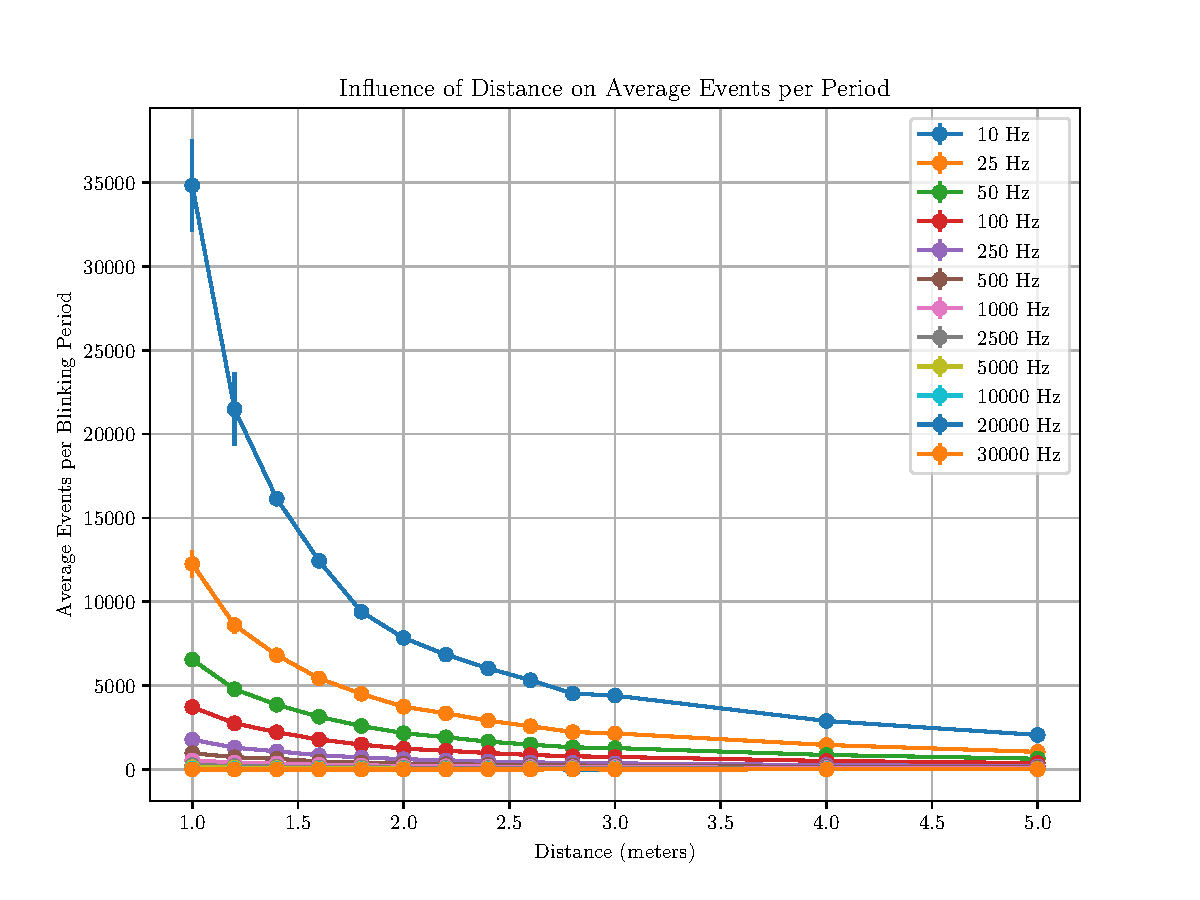
\includegraphics[width=0.5\textwidth]{./fig/semestral/dist.pdf}
%	  \label{fig:dist_1}
%	}
%	\subfloat[Influence of distance on the log of average number of events.] {
%	  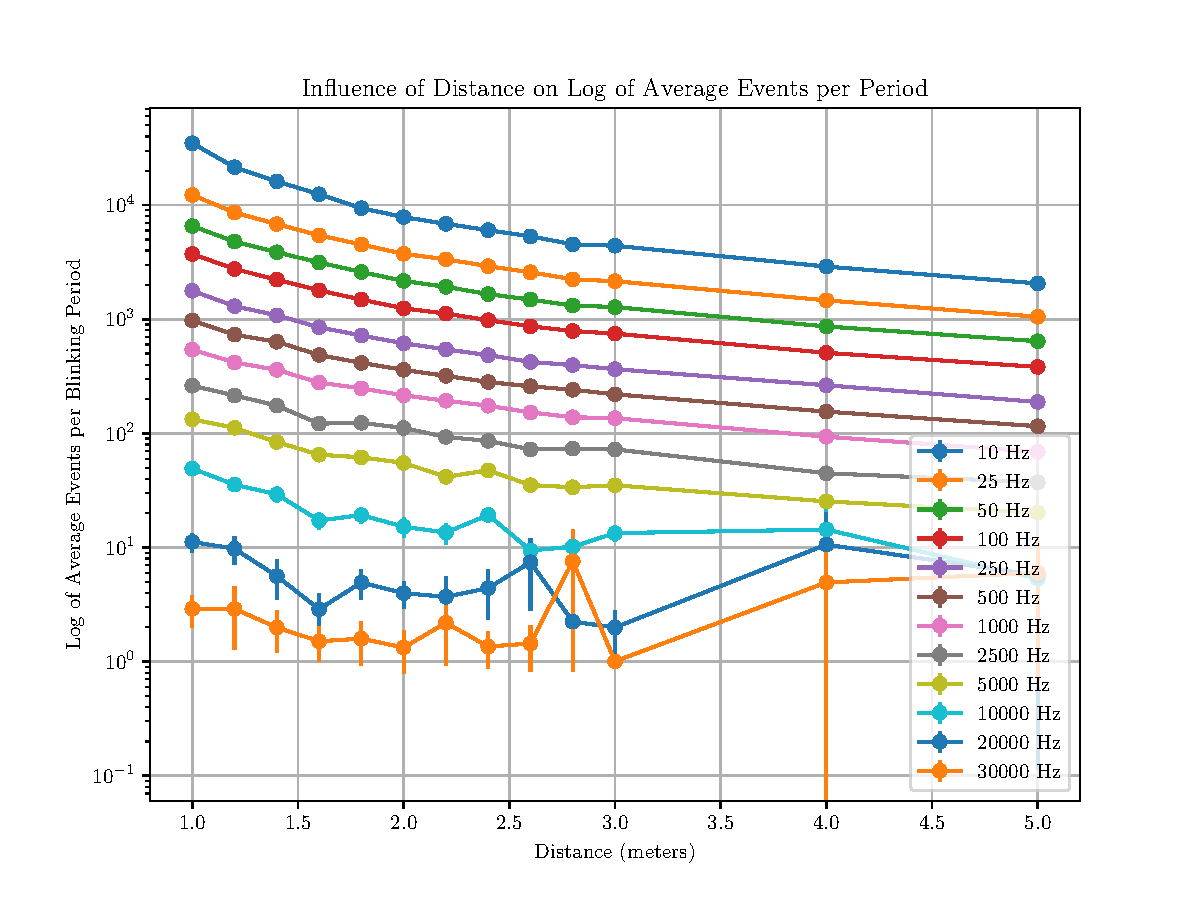
\includegraphics[width=0.5\textwidth]{./fig/semestral/distlog.pdf}
%	  \label{fig:dist_2}
%	}
%	\caption{
%  The influence of distance on the average number of events with the UAV rotated 0 degrees relative to the event-based camera on \reffig{fig:dist_1}, and with the log of the average number of events on \reffig{fig:dist_2}.
% }
%	\label{fig:dist}
%\end{figure}
%\begin{figure}[H]
%	\centering
%	\subfloat[Influence of frequency on the average number of events.] {
%	  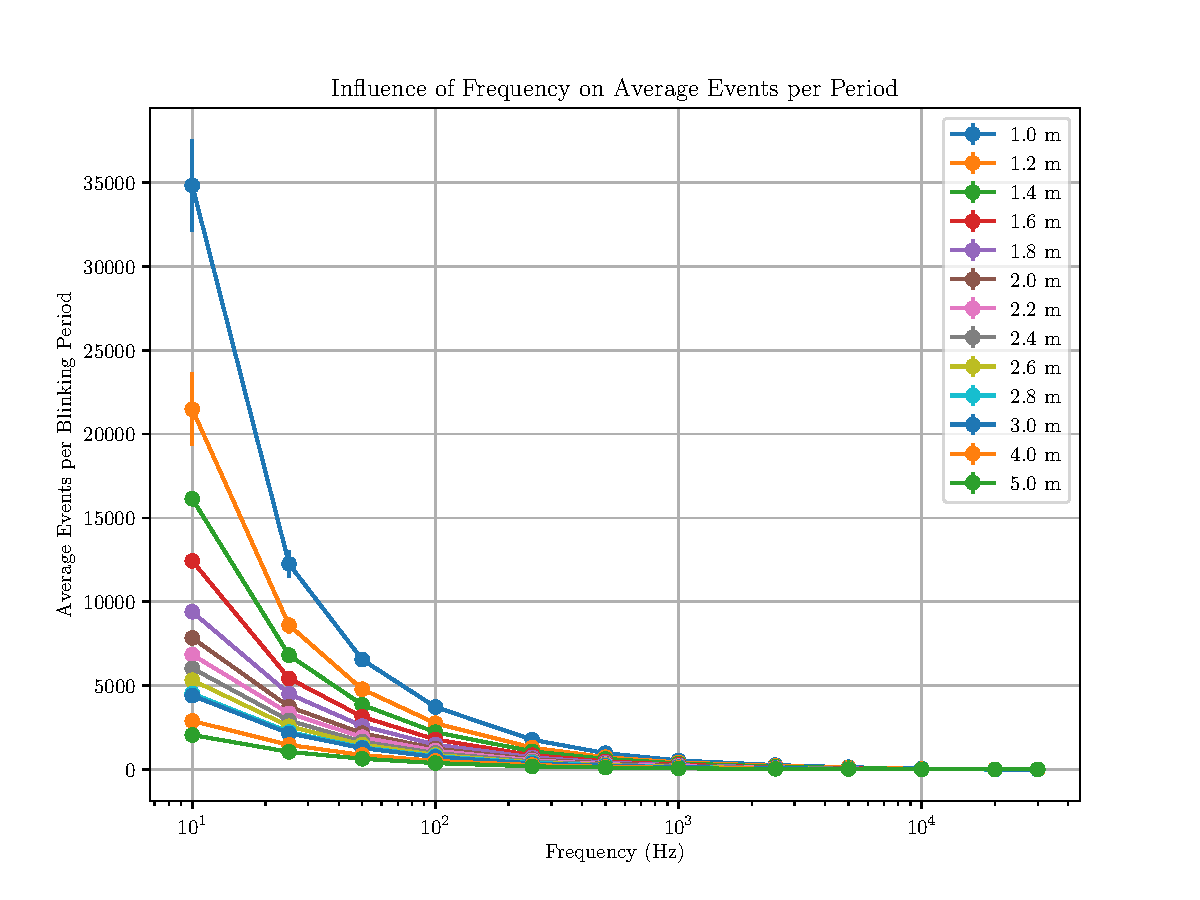
\includegraphics[width=0.5\textwidth]{./fig/semestral/freq.pdf}
%	  \label{fig:freqs_1}
%	}
%	\subfloat[Influence of frequency on the log of average number of events.] {
%	  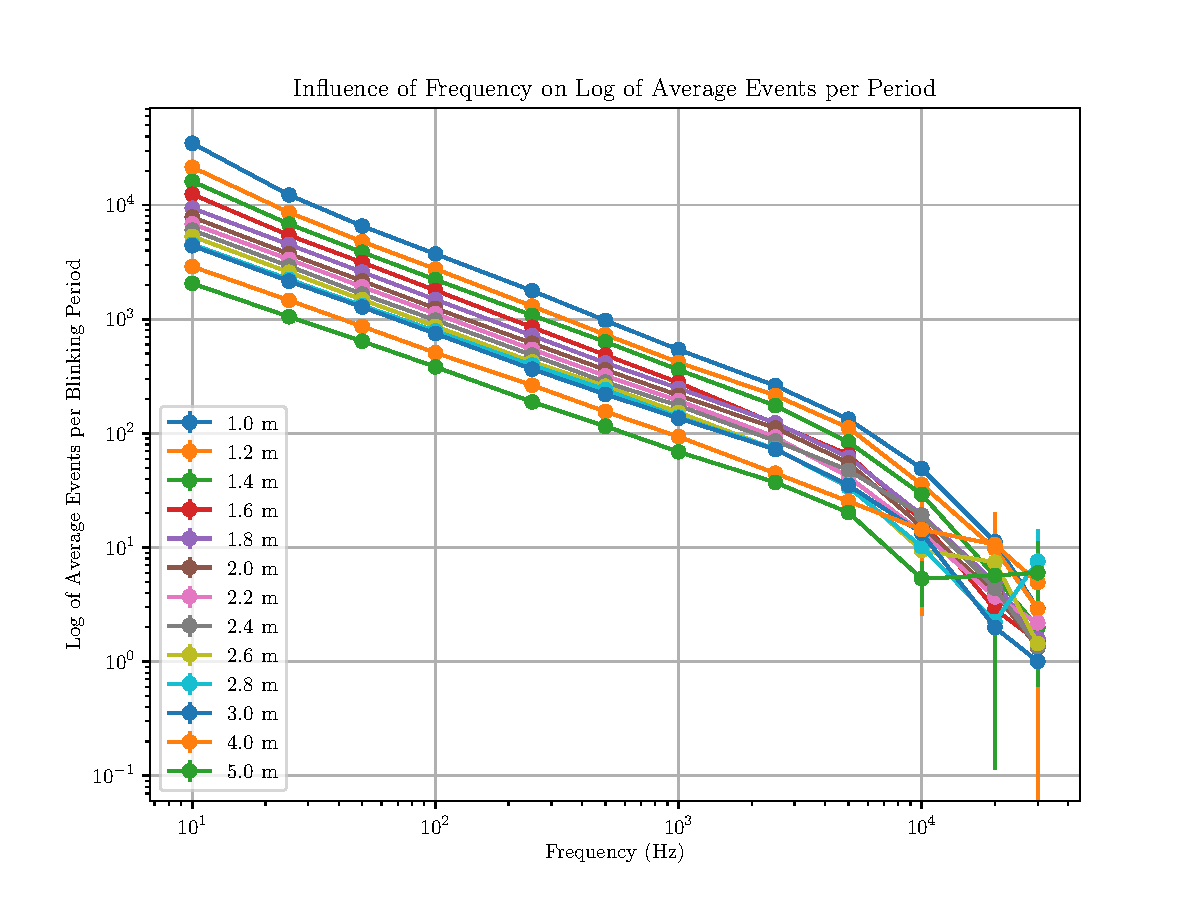
\includegraphics[width=0.5\textwidth]{./fig/semestral/freqlog.pdf}
%	  \label{fig:freqs_2}
%	}
%	\caption{
%  The influence of frequency on the average number of events with the UAV rotated 0 degrees relative to the event-based camera on \reffig{fig:freqs_1}, and with the log of the average number of events on \reffig{fig:freqs_2}.
%  }
%	\label{fig:freqs}
%\end{figure}

\begin{figure}[H]
    \centering
    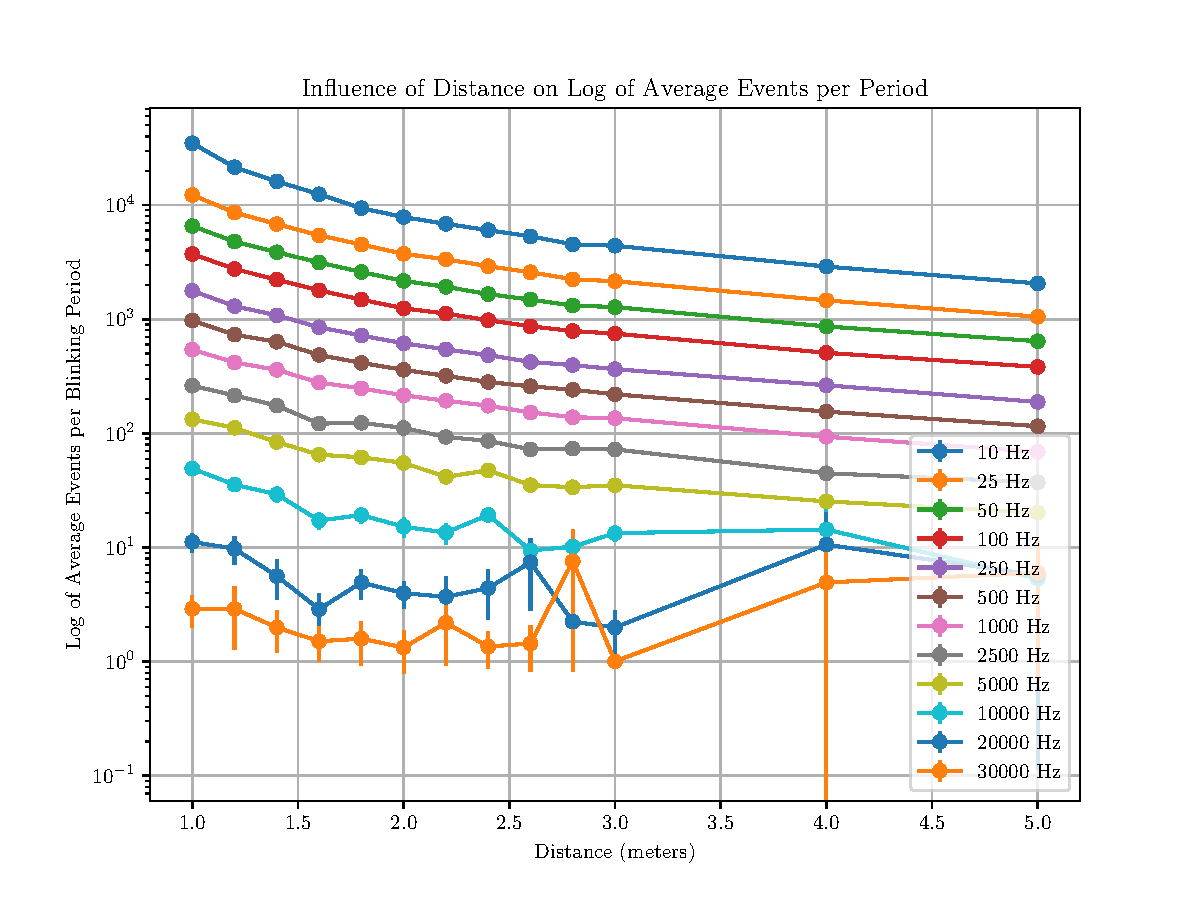
\includegraphics[width=0.85\textwidth]{./fig/semestral/distlog.pdf}
    \caption{
        Influence of distance on the log of the average number of events, with the UAV rotated 0 degrees relative to the event-based camera.
    }
    \label{fig:dist}
\end{figure}

\begin{figure}[H]
    \centering
    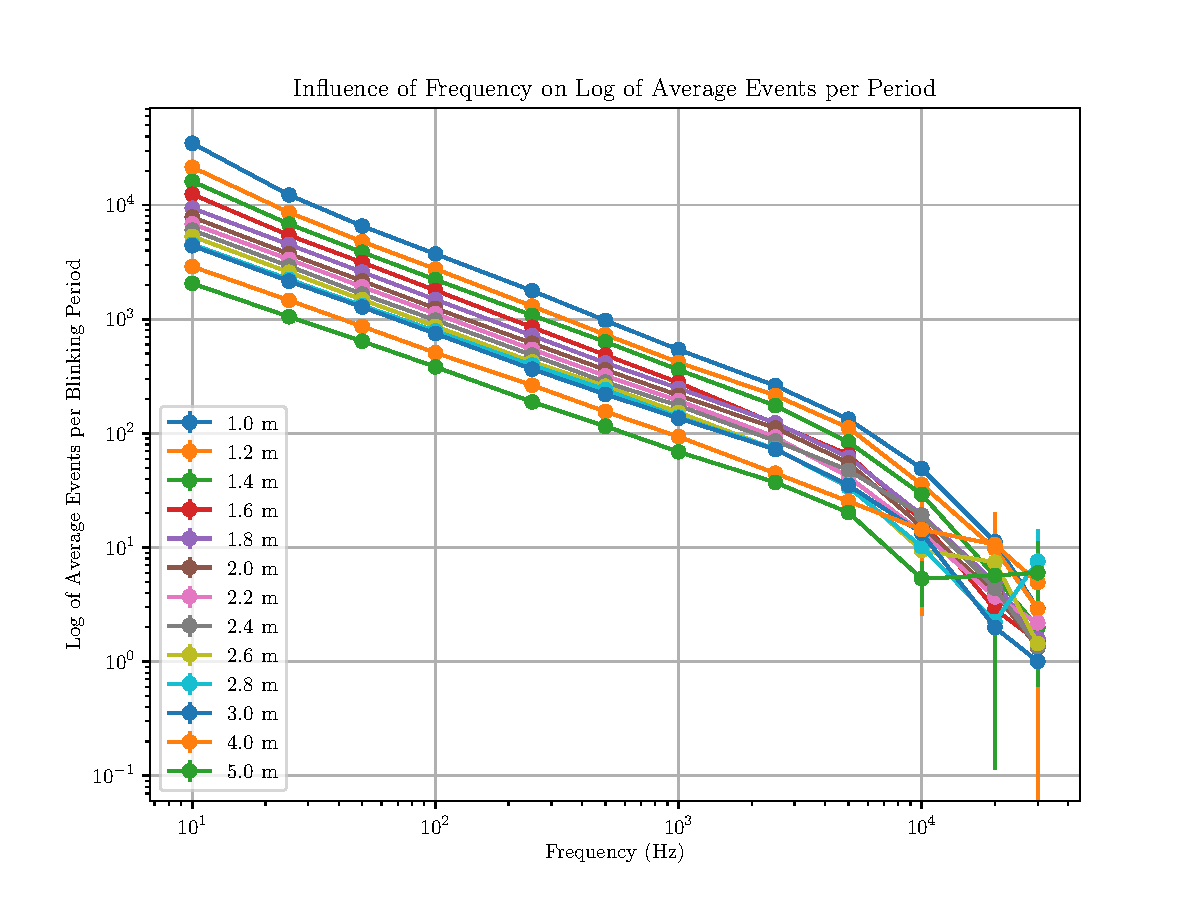
\includegraphics[width=0.85\textwidth]{./fig/semestral/freqlog.pdf}
    \caption{
        Influence of frequency on the log of the average number of events, with the UAV rotated 0 degrees relative to the event-based camera.
    }
    \label{fig:freqs}
\end{figure}

\begin{figure}[H]
    \centering
    \subfloat[$10$ Hz blinking frequency] {
        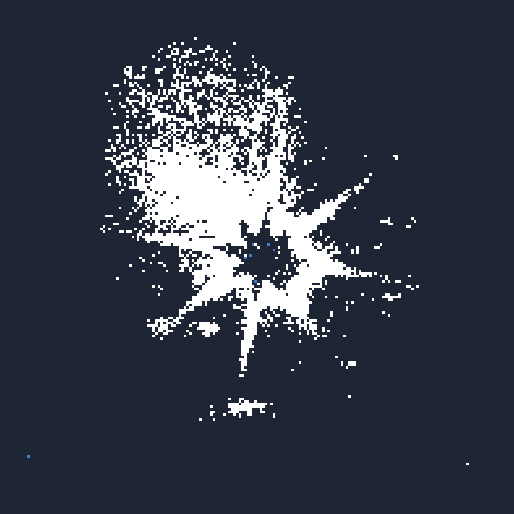
\includegraphics[width=0.3\textwidth]{./fig/photos/leds_freq/freq-1.jpg}
        \label{fig:freqsi_1}
    }
    \subfloat[$250$ Hz blinking frequency] {
        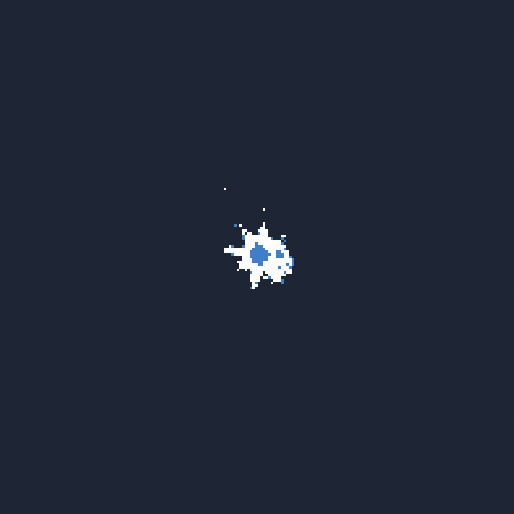
\includegraphics[width=0.3\textwidth]{./fig/photos/leds_freq/freq-2.jpg}
	  \label{fig:freqsi_2}
    }
    \subfloat[$2500$ Hz blinking frequency] {
        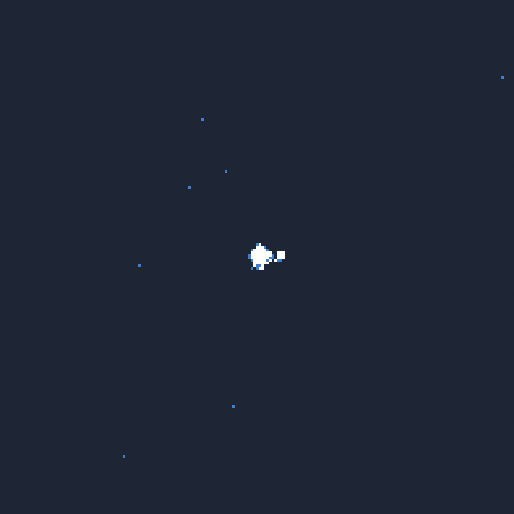
\includegraphics[width=0.3\textwidth]{./fig/photos/leds_freq/freq-3.jpg}
	  \label{fig:freqsi_3}
    }
    \caption{
        The influence of frequency on the perceived brightness of the \ac{LED}s, with blinking frequencies of $10$ Hz on \reffig{fig:freqsi_1}, $250$ Hz on \reffig{fig:freqsi_2} and $2500$ Hz on \reffig{fig:freqsi_3}.
    }
\label{fig:freqs_influence}
\end{figure}

For a selected frequency, the relationship between the average number of events and distance closely mirrors the inverse square
law \refeq{eq:inv_square_law}, a principle well known to describe how phenomena such as brightness, sound intensity, and electromagnetic field
diminish with the square of increasing distance.
As depicted in \reffig{fig:fit1}, when we plot the average number of events against distance, the data points align with this theoretical model.
This suggests that the number of events generated by the event-based camera is directly related to the brightness of the light source.

\begin{equation}
    \text{intensity} \propto \frac{1}{\text{distance}^2} .
    \label{eq:inv_square_law}
\end{equation}
While more complex functions could be used to fit the data, they would likely lead to overfitting rather than capturing the underlying trend in a generalizable way, thus the inverse square law provides a good approximation of the data.
\begin{figure}[H]
	\centering
	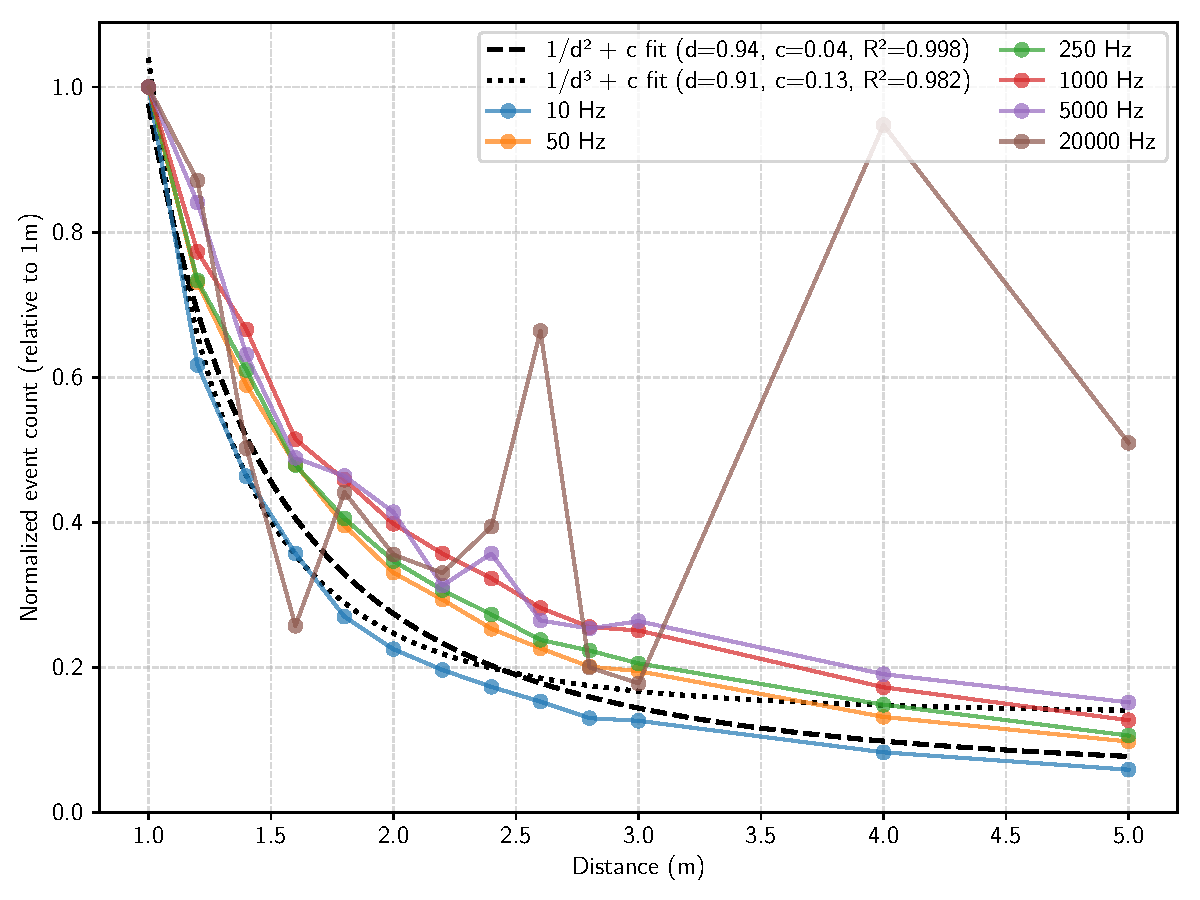
\includegraphics[width=0.70\textwidth]{./fig/pgfplot/build/inv_square.pdf}
	\caption{Experimental validation of the inverse square law}
	\label{fig:fit1}
\end{figure}

\subsection{Rotation angle influence}
From the manufacturer's datasheet of the used ProLight PM2B-1LLE 1W \ac{UV} Power \ac{LED} \footnote{The datasheet of ProLight PM2B-1LLE 1W UV Power LED can be obtained from \url{https://www.tme.eu/Document/9dfb498784ffdd07892a42f4f17c6f37/PM2B-1LLE-DTE.pdf}}
used in the UVDAR system, it can be learned, that the \ac{LED}s have a Lambertian radiation pattern,
which can be seen on \reffig{fig:lambertian}.
\begin {figure}[H]
	\centering
	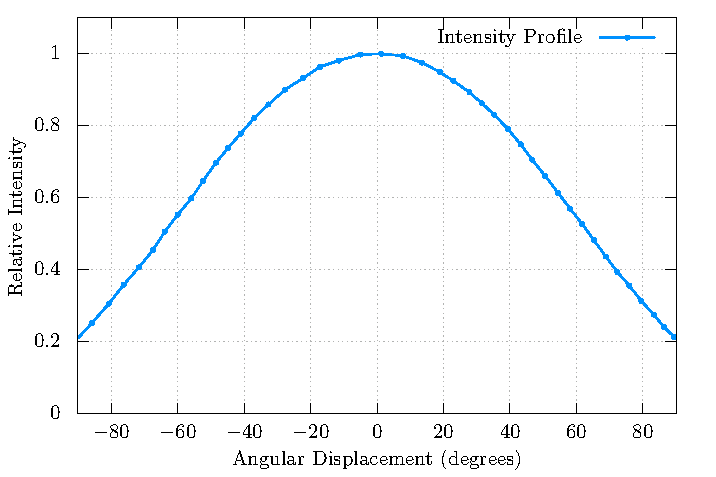
\includegraphics[width=0.75\textwidth]{./fig/semestral/lambertian/_new_lambertian.pdf}
	\caption{Lambertian radiation pattern of the PM2B-1LLE UV LED.}
	\label{fig:lambertian}
\end{figure}
This means that the intensity of the light emitted from the \ac{LED} decreases with the cosine
of the angle between the normal of the \ac{LED} and the direction of the light \refeq{eq:lambertian}.
\begin{equation}
	I(\theta) = I_0\cos(\theta)
	\label{eq:lambertian}
\end{equation}
To represent the whole end of the \ac{UAV} arm, two \ac{LED} sources need to be considered, orthogonal to each other.
This can be represented by shifting the previous distributions by $\pm 45$ degrees and adding them together. The 
theoretical distribution pattern of the light source is visible in \reffig{fig:lambert_combined}. 
The results extracted from the dataset of the \ac{UAV} rotations relative to the camera are shown in \reffig{fig:angles}.
\begin {figure}[H]
	\centering
	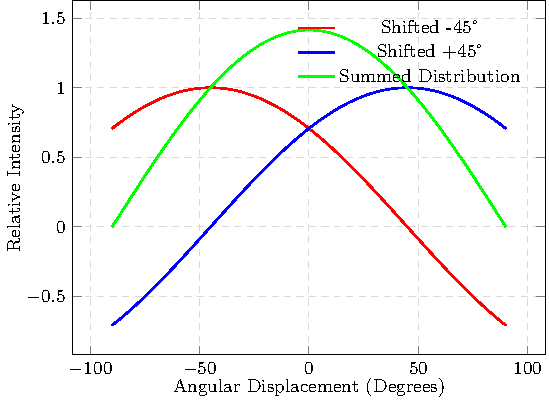
\includegraphics[width=0.60\textwidth]{./fig/semestral/lambertian/3lambertian.pdf}
	\caption{Radiation pattern of two lambertian light sources shifted by $\pm 45$ degrees.}
	\label{fig:lambert_combined}
\end{figure}

\begin{figure}[H]
	\centering
	\subfloat[Influence of rotation of the UAV on the log of average number of events at 0.5 m.] {
	  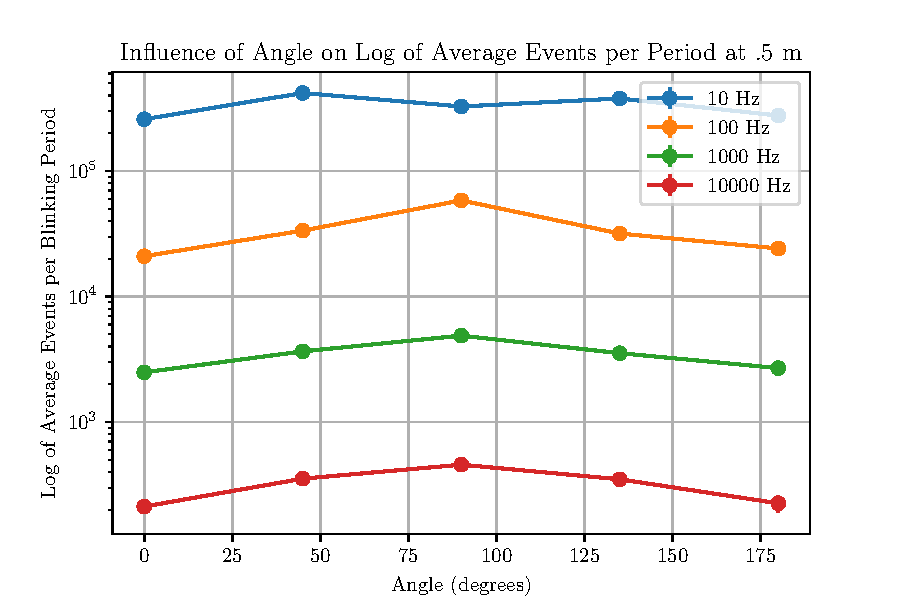
\includegraphics[width=0.5\textwidth]{./fig/semestral/angle1.pdf}
	  \label{fig:angle_1}
	}
	% \subfloat[Influence of rotation of the UAV on the log of average number of events at 1 m.] {
	%   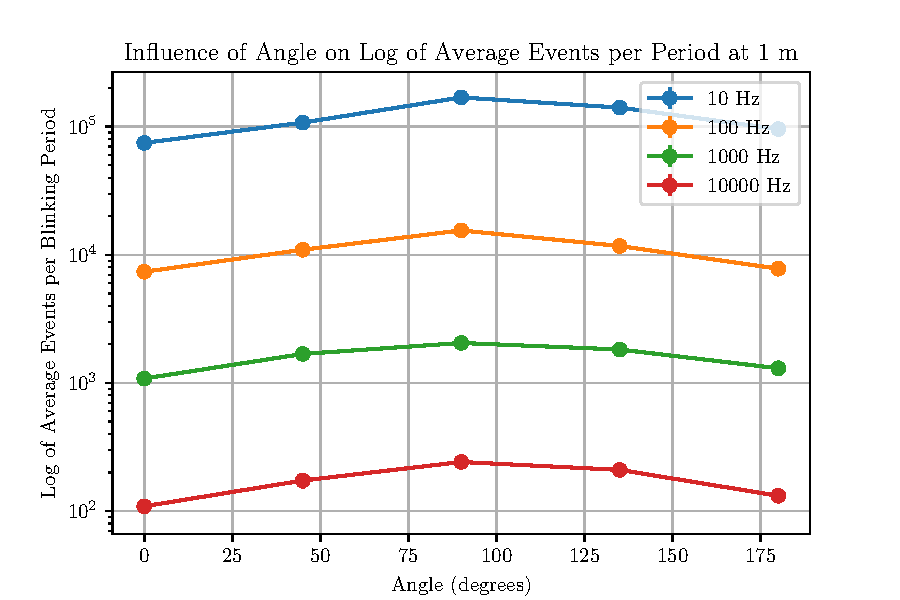
\includegraphics[width=0.5\textwidth]{./fig/semestral/angle2.pdf}
	%   \label{fig:angle_2}
	% }
	\subfloat[Influence of rotation of the UAV on the log of average number of events at 2 m.] {
	  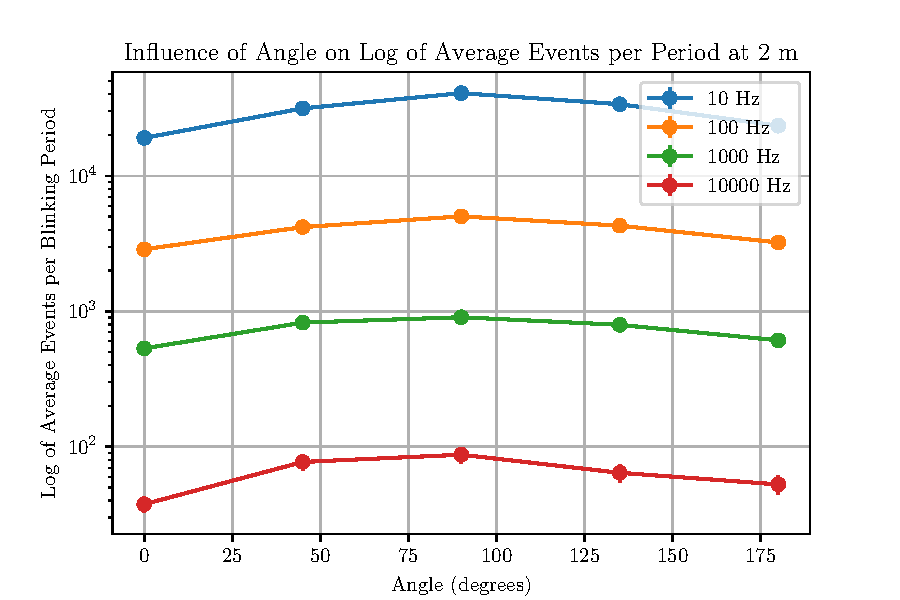
\includegraphics[width=0.5\textwidth]{./fig/semestral/angle3.pdf}
	  \label{fig:angle_3}
	}
	\caption{
  The influence of rotation angle on the log of average number of events at 0.5 m on \reffig{fig:angle_1} and at 2 m on \reffig{fig:angle_3}.
  }
	\label{fig:angles}
\end{figure}
The data show a rough approximation of the theoretical distribution on \reffig{fig:lambert_combined},
but with a drop of intensity at the middle of the distribution. This could be caused
by the fact that \ac{LED}s, when close to the camera, can be perceived as multiple light sources,
but when moved further away, they merge into one source as shown on \reffig{fig:leds}.

\begin{figure}[H]
	\centering
	\subfloat[2 LEDs with blinking frequency of 10 Hz at 0.5 m.] {
	  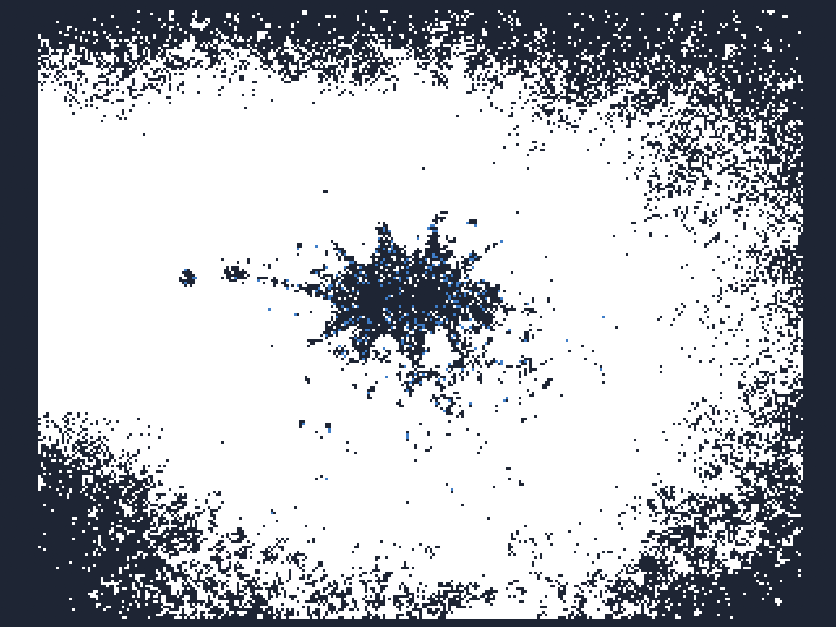
\includegraphics[width=0.5\textwidth]{./fig/photos/2leds_05m.png}
	  \label{fig:leds_1}
	}
	\subfloat[2 LEDs with blinking frequency of 10 Hz at 2 m.] {
	  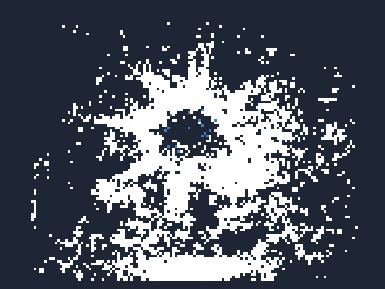
\includegraphics[width=0.5\textwidth]{./fig/photos/2leds_2m.png}
	  \label{fig:leds_2}
	}
	\caption{
  The light source on one arm of the UAV, consisting of two UV LEDs, blinking at a frequency of 10 Hz,
  placed at 0.5 m on \reffig{fig:leds_1} and 2 m at \reffig{fig:leds_2}.
  }
	\label{fig:leds}
\end{figure}
What can also be observed from \reffig{fig:leds} are the star-like shapes of the LEDs, which are supposed to be circular.
Those shapes are caused by light diffraction (and are named diffraction spikes), which are, in turn, caused by the aperture
blades in the lens of the camera. The number
of star spikes depends on the number of blades, the set aperture and the light source intensity then causes stars of different
levels of profoundness~\cite{lendermann2018computational}. This can be observed by comparing how profound the star shapes are on different
frequencies, as shown on \reffig{fig:stars}.

\begin{figure}[H]
	\centering
	\subfloat[LED blinking at 10 Hz at 1.0 m] {
	  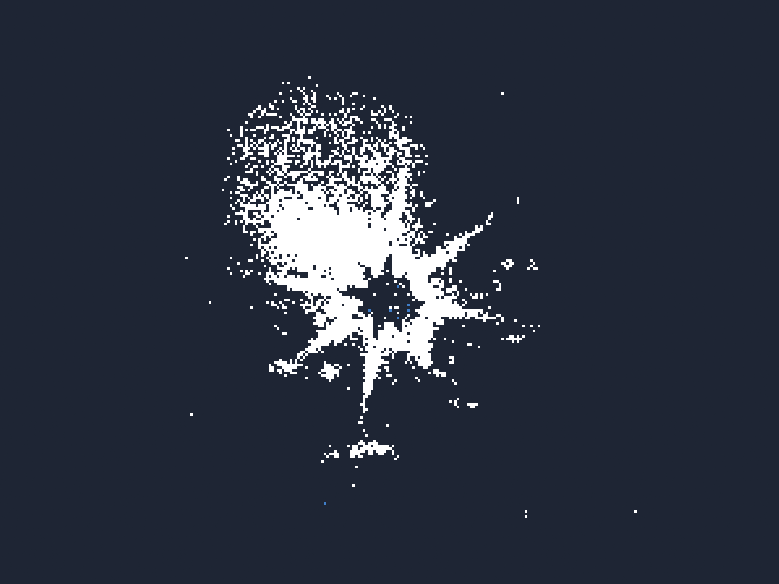
\includegraphics[width=0.5\textwidth]{./fig/photos/led_10hz.png}
	  \label{fig:stars_1}
	}
	\subfloat[LED blinking at 1 kHz at 1.0 m] {
	  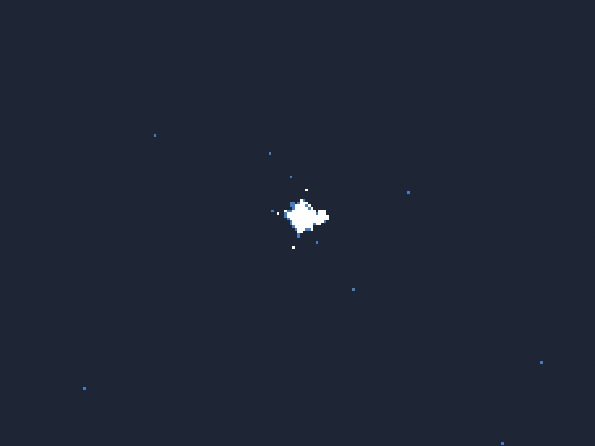
\includegraphics[width=0.5\textwidth]{./fig/photos/led_1000hz.png}
	  \label{fig:stars_2}
	}
	\caption{
  Two same LED light sources at 1.0 meters, blinking at 10 Hz and 1 kHz.
  \reffig{fig:stars_1} shows a visible diffraction star (while being much brighter), while \reffig{fig:stars_2} shows a
  much more cicular source of light that is not as bright.
  }
	\label{fig:stars}
\end{figure}

% ============= Calibration results ================

\newpage
\section{Calibration results}

The camera calibration was performed on a series of images, where the calibration lattice was placed as various angles and distances from the camera.
For ideal calibration results, the lattice should be placed in all visible parts of the image, as the distortion of the fisheye is more pronounced at the edges
of the visible area. The calibration was performed on a polynomial of degree 4, more would lead to overfitting and is also not necessary.
The calibration results can be seen in \reffig{fig:calib_r}.

\begin{figure}[H]
	\centering
	\subfloat[Calibrated lens model function] {
	  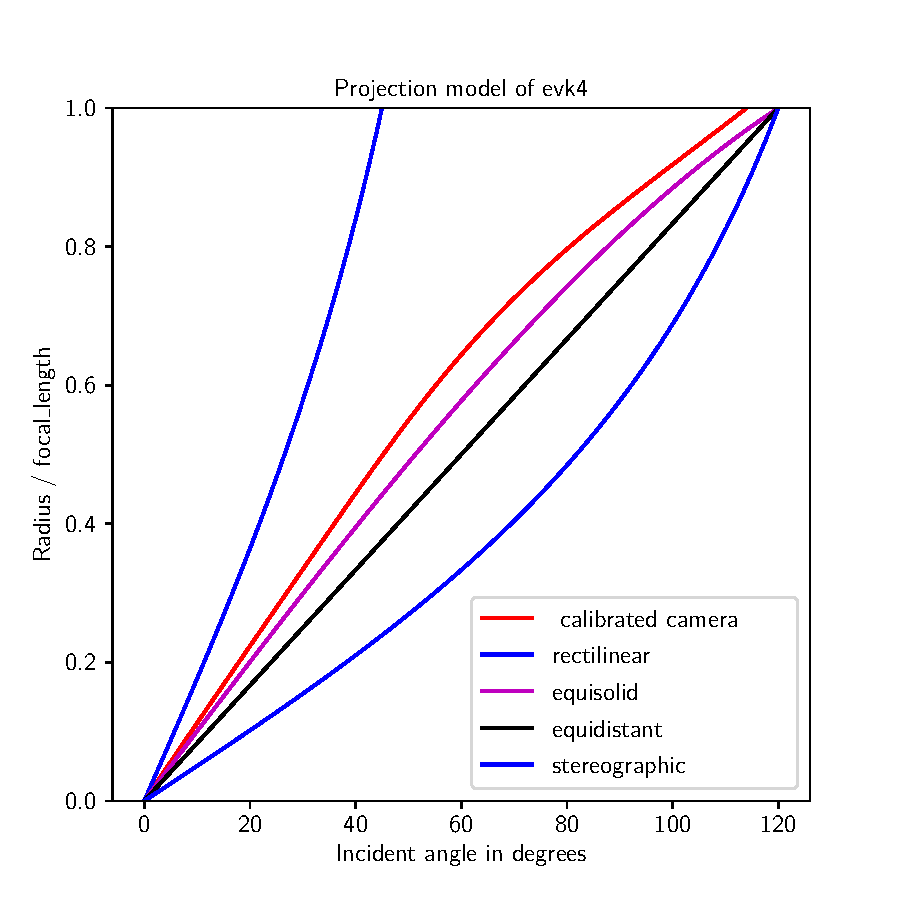
\includegraphics[width=0.49\textwidth]{./fig/pgfplot/build/evk4_projection_new.pdf}
	  \label{fig:calib_r_1}
	}
	\subfloat[Calibration images mean reprojection errors] {
	  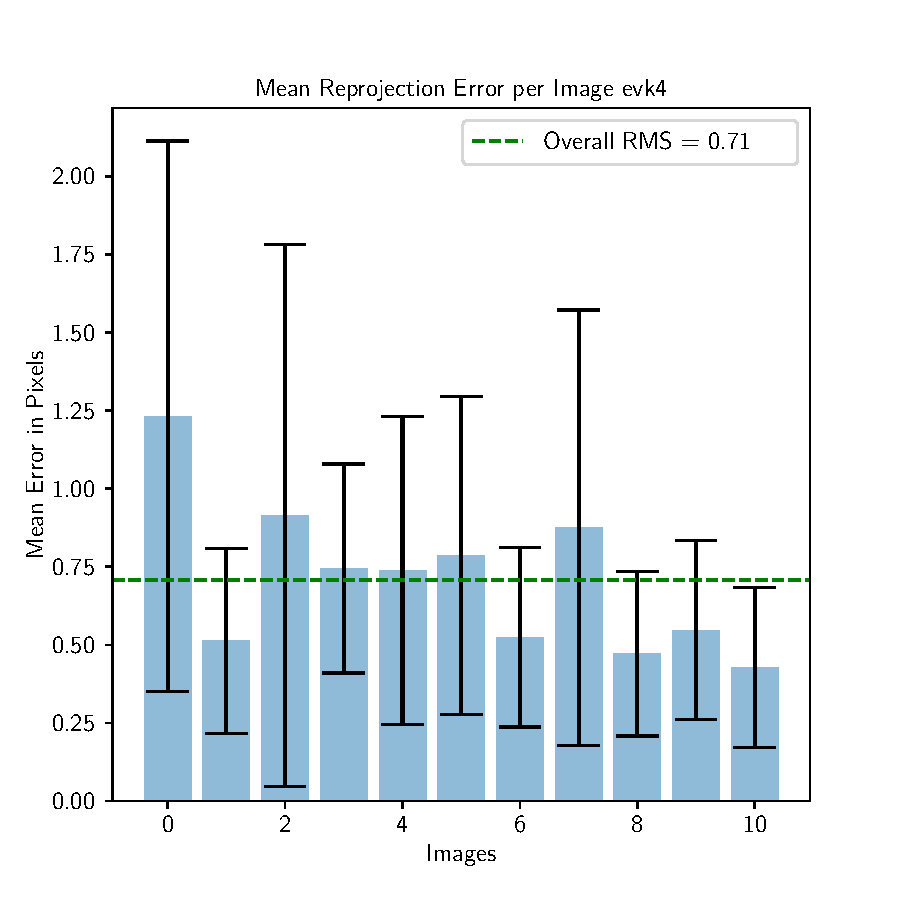
\includegraphics[width=0.49\textwidth]{./fig/pgfplot/build/evk4_reprojection_error_new.pdf}
	  \label{fig:calib_r_2}
	}
	\caption{
		Calibration results with the calibrated lens model function highlighted in red in \reffig{fig:calib_r_1} and the calibration images mean reprojection errors on \reffig{fig:calib_r_2}.
  }
	\label{fig:calib_r}
\end{figure}

The problem of fitting a minimal encompassing ellipse to event data, in order to get the visible area of the camera sensor, can be formulated
as an unconstrained optimization problem \ref{eq:ellipse_opt}, where we minimize the squared distances of convex hull points to the ellipse boundary.
% of minimizing the sum of point distances, that lie outside of the
%ellipse, while minimizing the ellipse parameters $a$, $b$.
The optimized ellipse can be seen in \reffig{fig:ellipse_fit}.
\begin{equation}
(a^*, b^*) = \underset{a, b > 0}{\text{argmin}} \quad \sum_{(x_i,y_i) \in \mathcal{H}} \left( \frac{x_i^2}{a^2} + \frac{y_i^2}{b^2} - 1 \right)^2
\label{eq:ellipse_opt}
\end{equation}
\text{where} $\mathcal{H} = \text{Conv}\{(x_i,y_i)\}_{i=1}^n$ is the set of points in the convex hull of generated events.

%\begin{figure}[H]
%	\centering
%	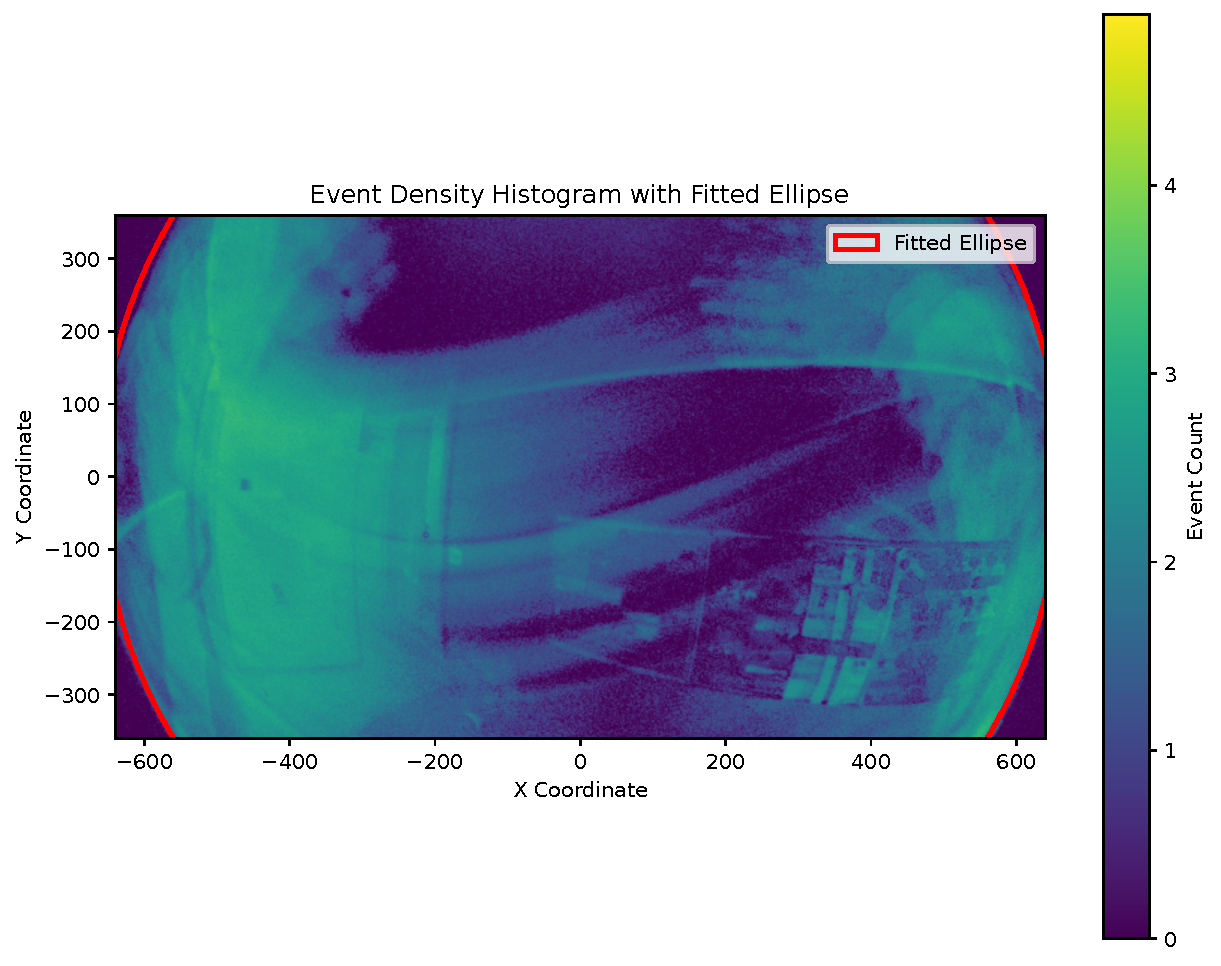
\includegraphics[width=0.65\textwidth]{./fig/svg/ellipse_fit.pdf}
%	\caption{Fitted ellipse to the calibration data, with semi-major axis $a^* = 652$, and semi-minor axis $b^* = 650$.}
%	\label{fig:ellipse_fit}
%\end{figure}
\begin{figure}[H]
	\centering
	\subfloat[Fitted ellipse.] {
	  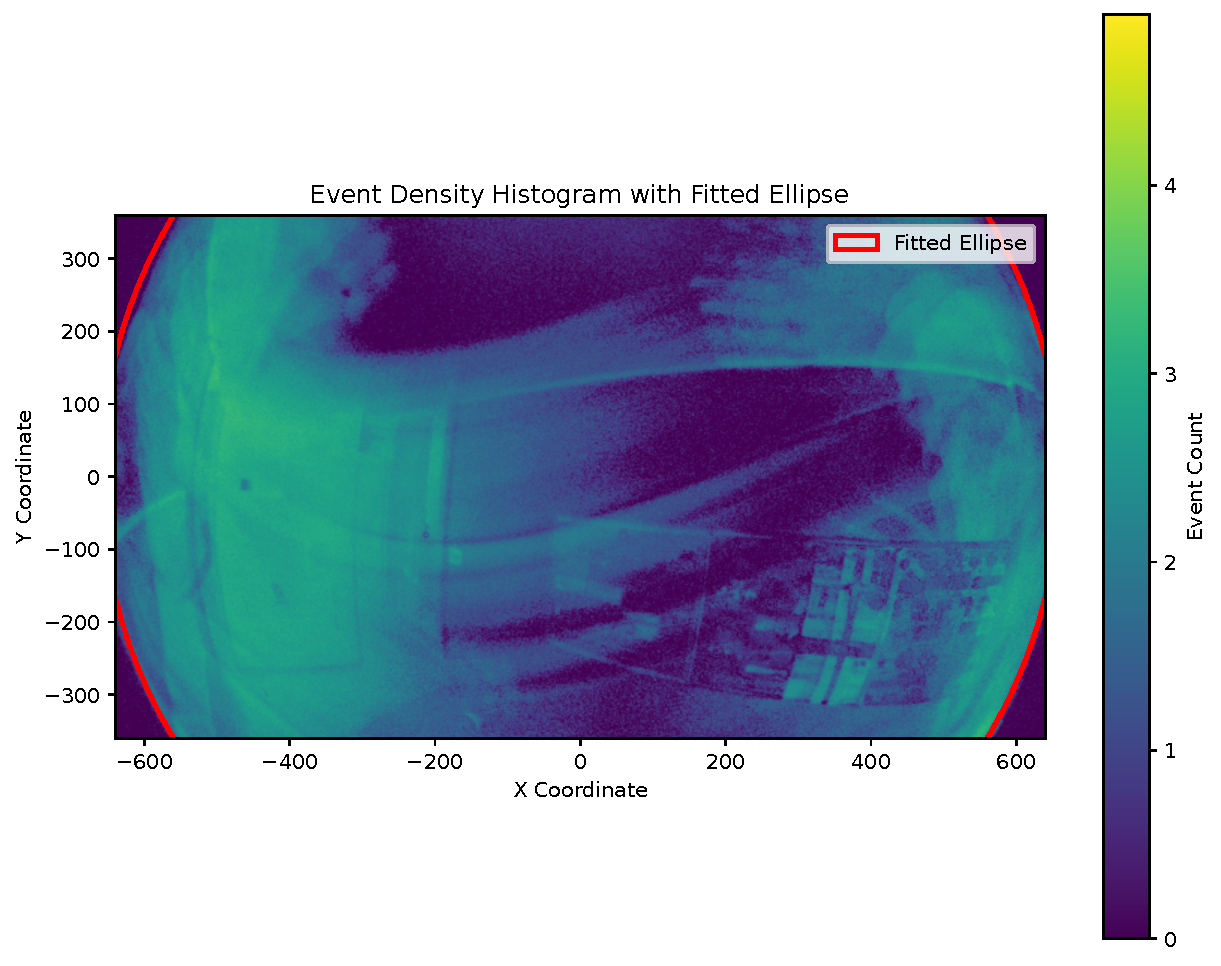
\includegraphics[width=0.5\textwidth]{./fig/svg/ellipse_fit.pdf}
	  \label{fig:ellipse_fit_1}
	}
	\subfloat[Events with convex hull points] {
	  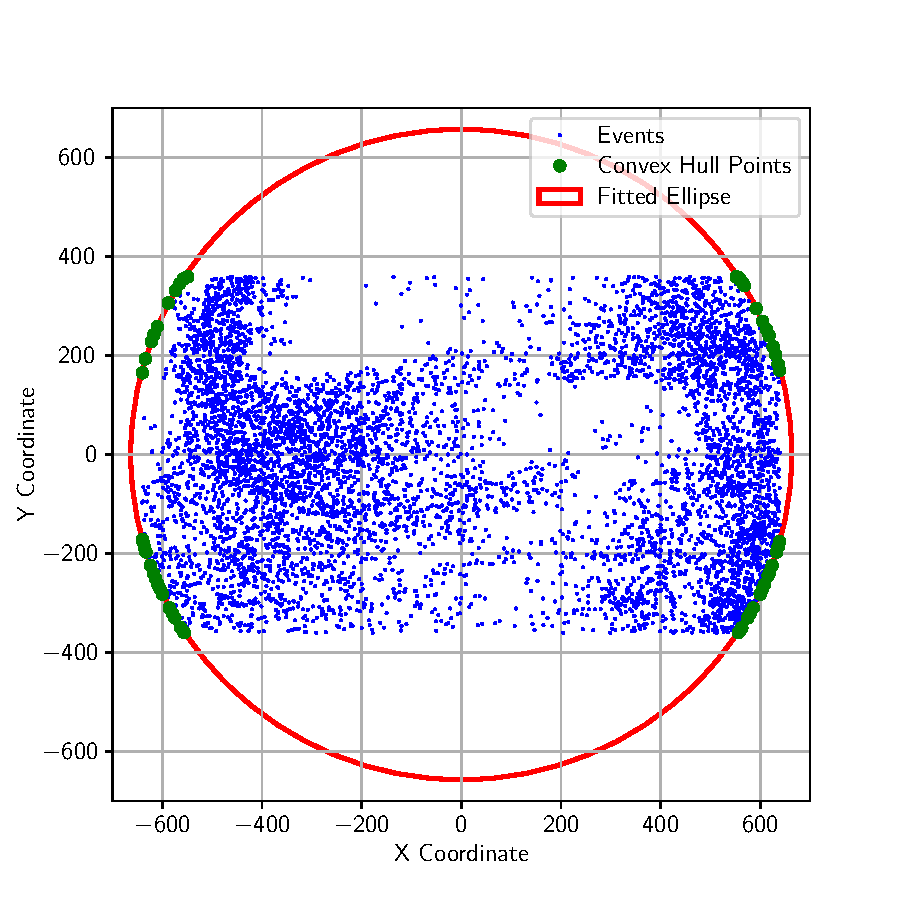
\includegraphics[width=0.45\textwidth]{./fig/pgfplot/build/ellipse_hull.pdf}
	  \label{fig:ellipse_fit_2}
	}
	\caption{
		Fitted ellipse to the calibration data, with semi-major axis $a^* = 663$, and semi-minor axis $b^* = 657$
        on \reffig{fig:ellipse_fit_1} with separated convex hull points in green on \reffig{fig:ellipse_fit_2}.
  }
	\label{fig:ellipse_fit}
\end{figure}

Finally, to visualize the calibration results, we map every point from the image plane using the \texttt{cam2world}\footnote{\url{https://github.com/jakarto3d/py-OCamCalib/blob/main/src/pyocamcalib/modelling/camera.py}}
function from \texttt{py-OCamCalib}, which takes a 2D image point, and returns
the corresponding 3D optical ray on the camera's unit sphere. For each point, we calculate its angle from the optical axis (a vector $\mathbf{v} = \begin{bmatrix} 0 & 0 & 1 \end{bmatrix}^{T}$),
and mask out the visible area with the ellipse fitted in \reffig{fig:ellipse_fit}. We can see the results in \reffig{fig:calibration_viz}.

\begin{figure}[H]
	\centering
	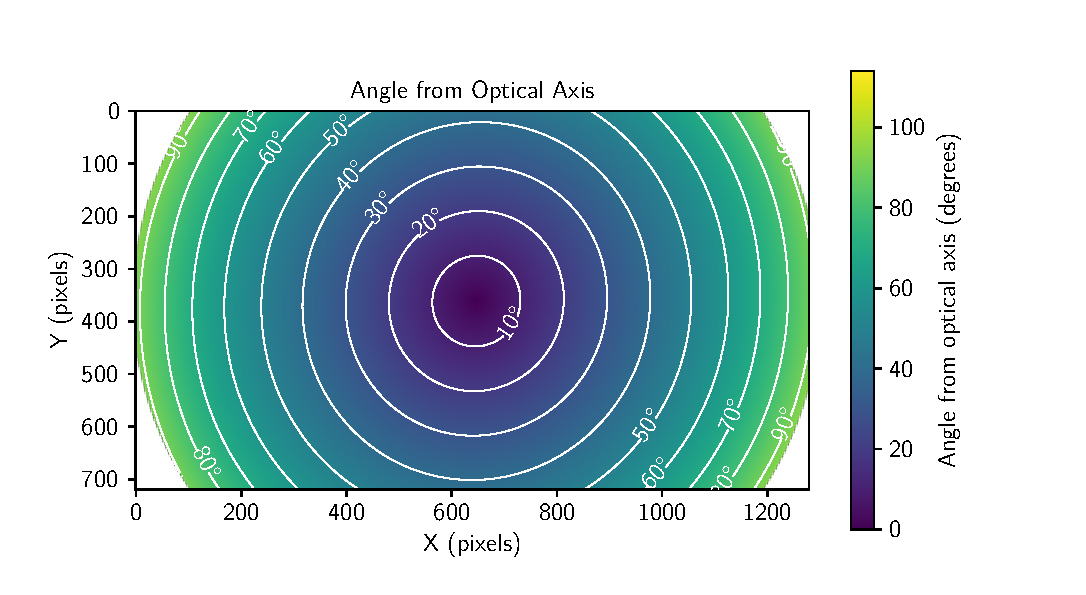
\includegraphics[width=1.0\textwidth]{./fig/pgfplot/build/evk4_viz.pdf}
	\caption{Angle from optical axis visualization, with the maximum angle of 93.47 degrees.}
	\label{fig:calibration_viz}
\end{figure}

We can also apply a perspective conversion to the whole image, which now correctly represents distances and angles. We can notice this by looking
at the calibration lattice at \reffig{fig:calib_c}, which now looks like a grid of points.

\begin{figure}[H]
	\centering
	\subfloat[Uncalibrated image.] {
	  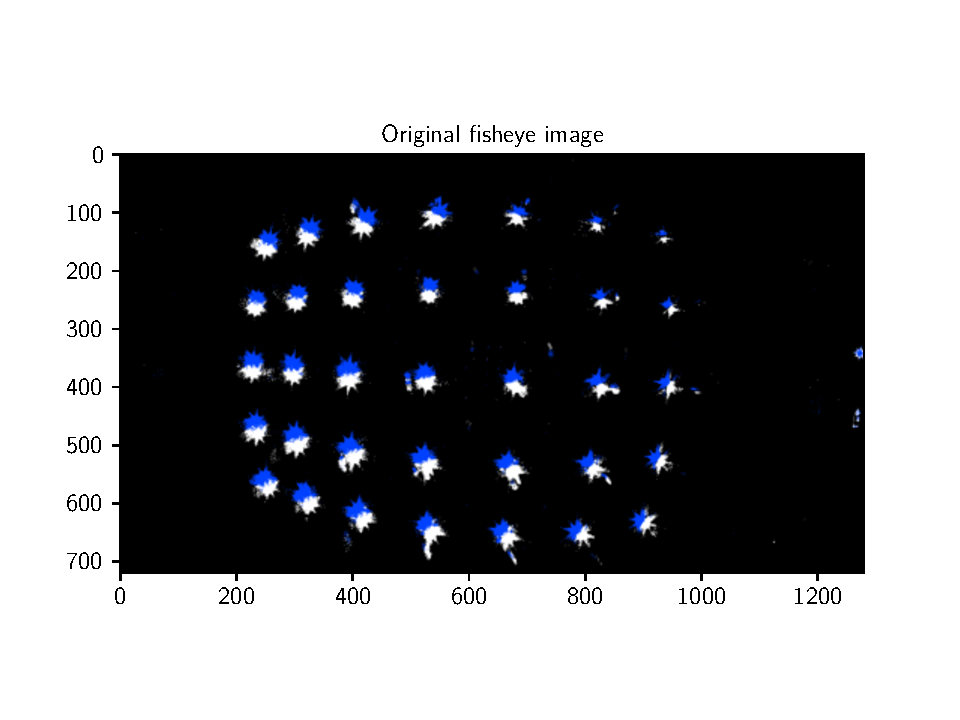
\includegraphics[width=0.5\textwidth]{./fig/pgfplot/build/image_uncalib.pdf}
	  \label{fig:calib_c_1}
	}
	\subfloat[Calibrated image.] {
	  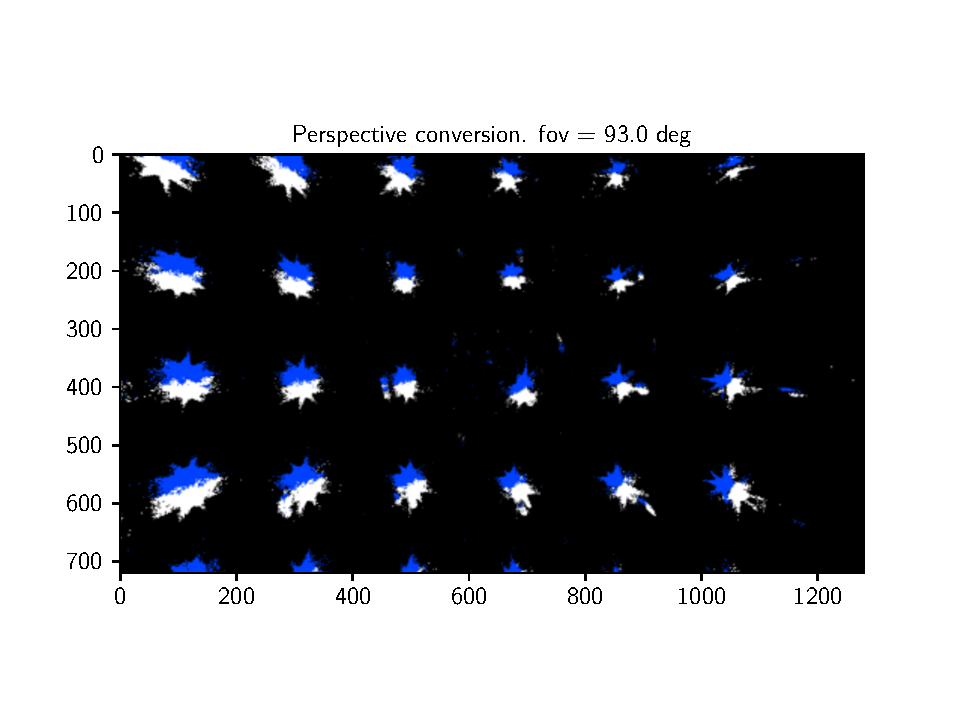
\includegraphics[width=0.5\textwidth]{./fig/pgfplot/build/image_calib.pdf}
	  \label{fig:calib_c_2}
	}
	\caption{
		Two photos of the calibration lattice, one uncalibrated on \reffig{fig:calib_c_1} and the other calibrated at \reffig{fig:calib_c_2}, which does not
		exhibit any distortion.
  }
	\label{fig:calib_c}
\end{figure}

For the calibration of the Entaniya $280$ degree lens a classical chessboard target was used, as the precise localization of the blob centers proved to be nearly impossible while using the \ac{LED} lattice calibration target. The corners of the chessboard pattern provide
better contrast and allow for precise localization of the center; unfortunately, they need to be labeled manually in this case as seen in \reffig{fig:calib_ent_label}.
The calibration results can be seen on \reffig{fig:calib_e}, with the visualization on \reffig{fig:calib_ent_viz} and the perspective projection on
\reffig{fig:calib_ent_proj}.
\begin{figure}[htbp]
	\centering
	%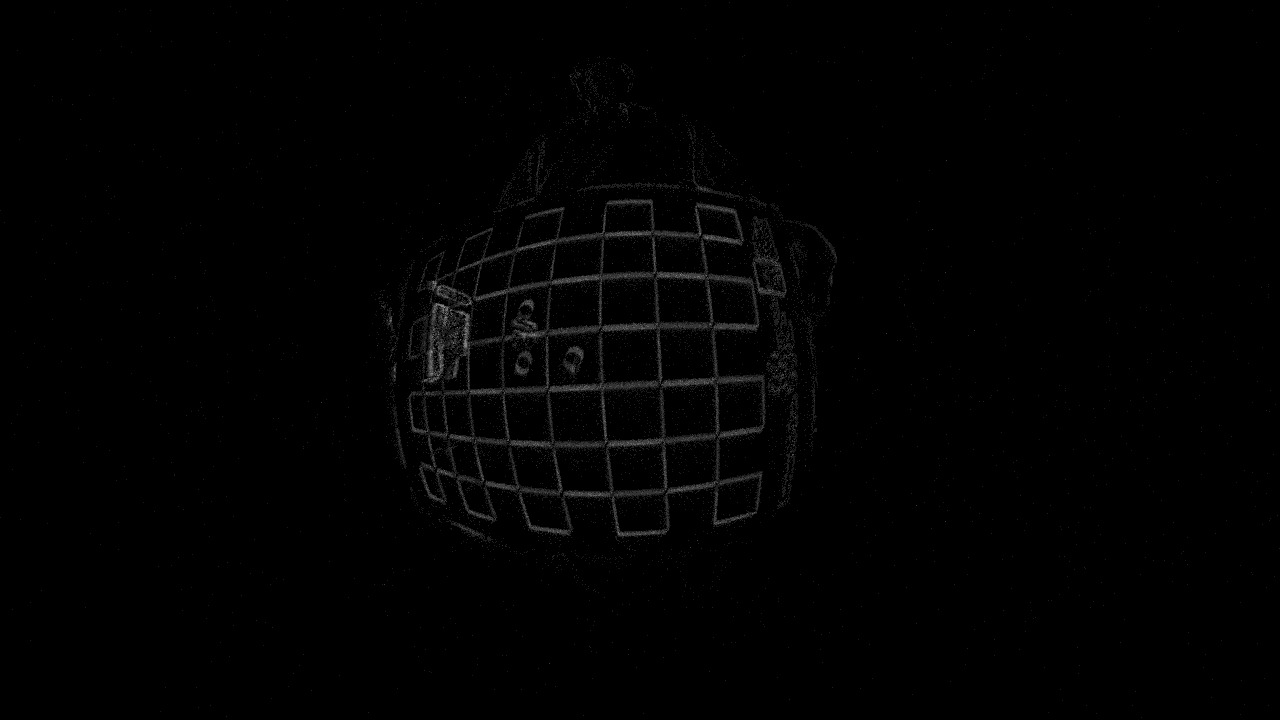
\includegraphics[width=0.6\textwidth]{./fig/photos/frame_58CEE7E0.png}
        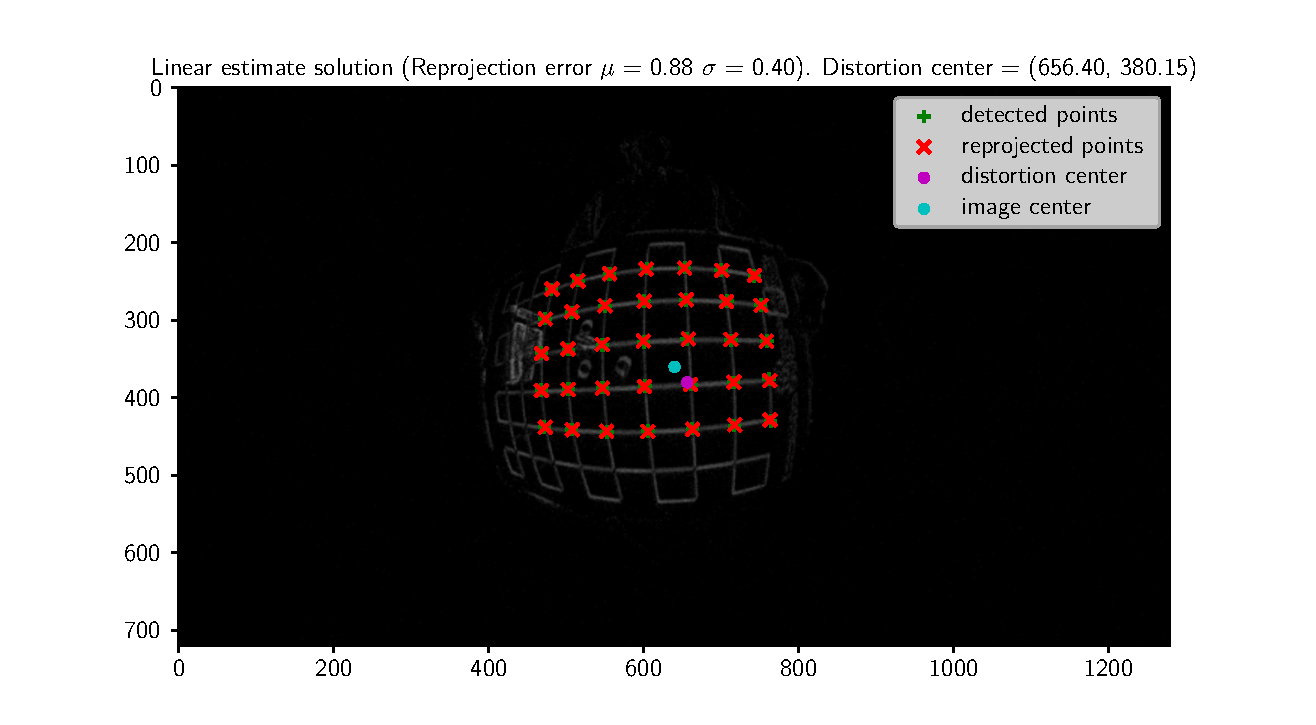
\includegraphics[width=0.8\textwidth]{./fig/pgfplot/build/chessboard_280.pdf}
	\caption{Chessboard calibration target visible in 280 degree lens with marked chessboard edge points}
	\label{fig:calib_ent_label}
\end{figure}

\begin{figure}[H]
	\centering
	\subfloat[Calibrated lens model function] {
	  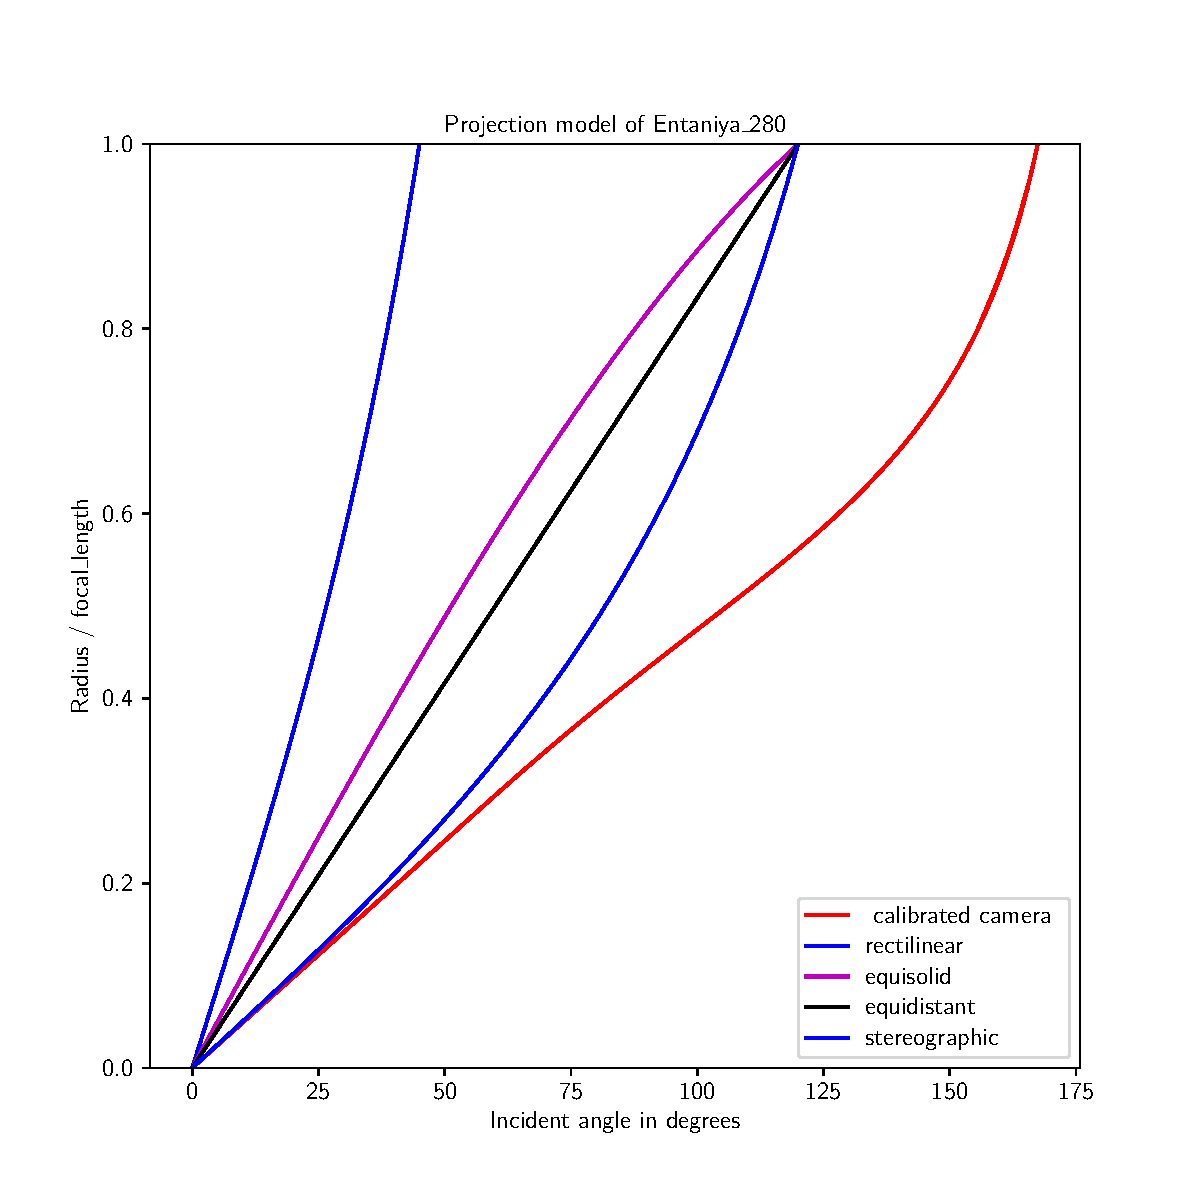
\includegraphics[width=0.5\textwidth]{./fig/pgfplot/build/proj_280_new.pdf}
	  \label{fig:calib_e_1}
	}
	\subfloat[Calibration images mean reprojection errors] {
	  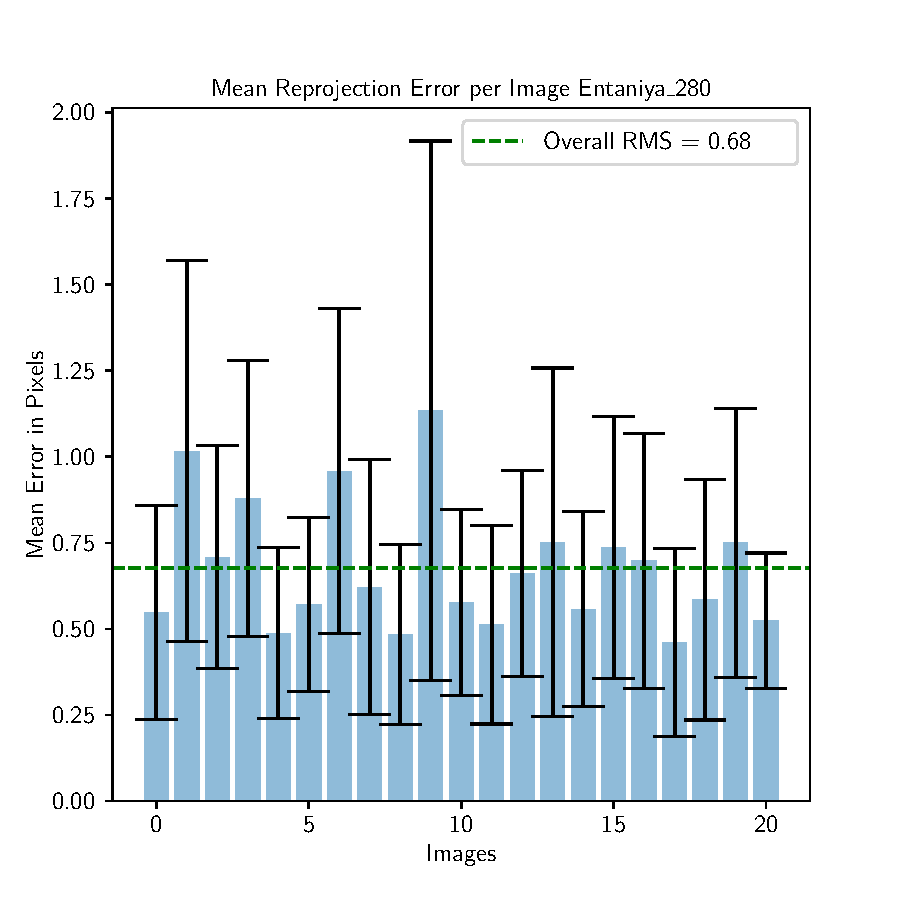
\includegraphics[width=0.5\textwidth]{./fig/pgfplot/build/err_280_new.pdf}
	  \label{fig:calib_e_2}
	}
	\caption{
		Calibration results for the Entaniya 280 degree lens with the calibrated lens model function highlighted in red in \reffig{fig:calib_e_1} and the calibration images mean reprojection errors on \reffig{fig:calib_e_2}.
  }
	\label{fig:calib_e}
\end{figure}
\begin{figure}[H]
	\centering
	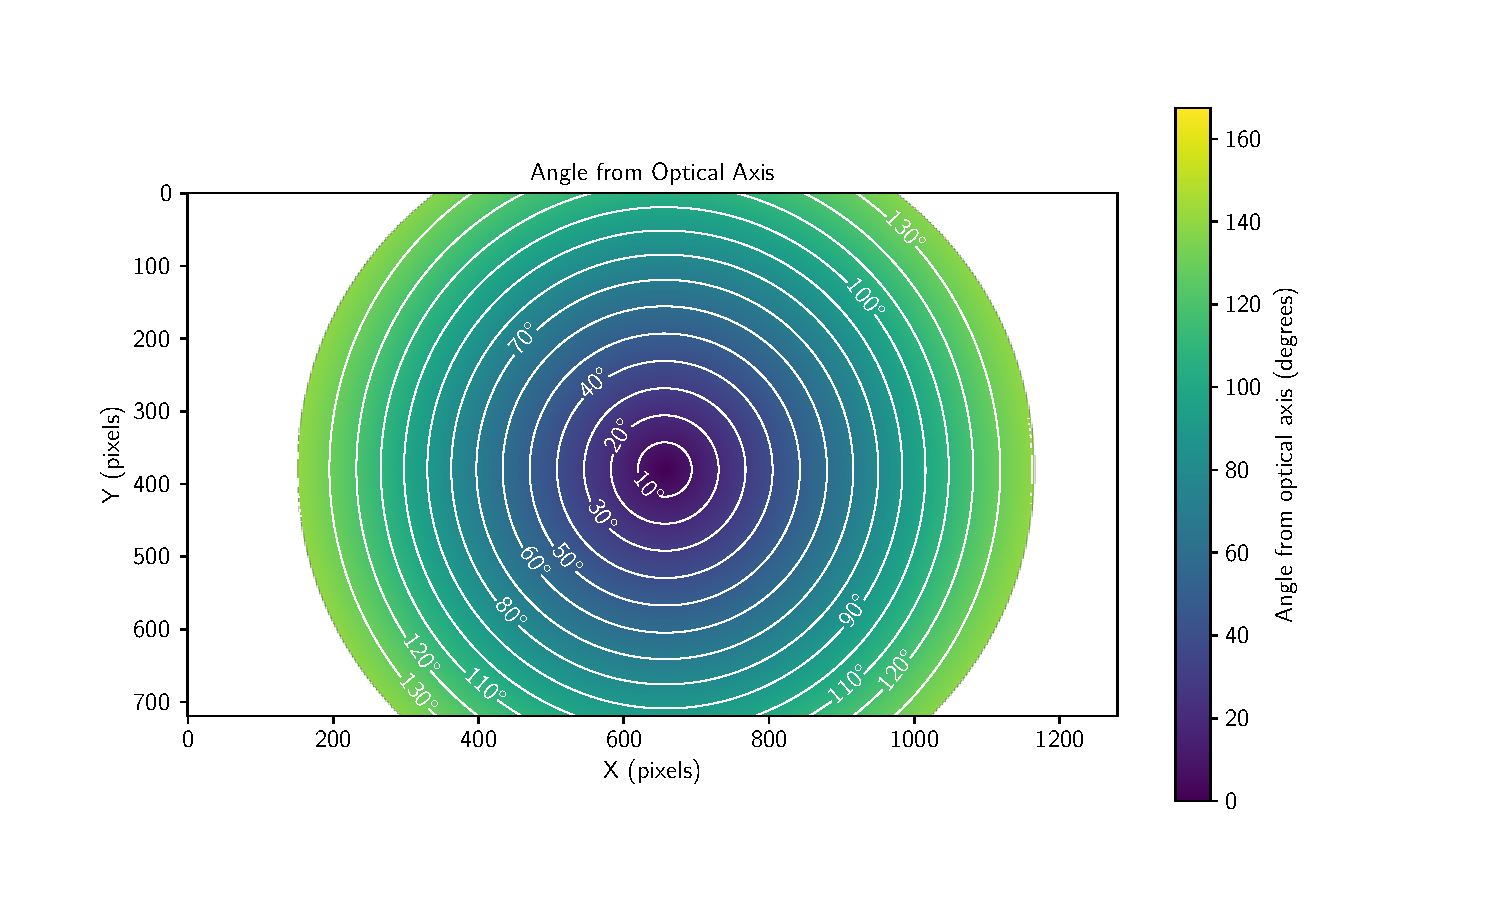
\includegraphics[width=1.0\textwidth]{./fig/pgfplot/build/viz_ent.pdf}
	\caption{Angle from optical axis visualization, with the maximum angle of 140 degrees on each side, making its \ac{FOV} 280 degrees.}
	\label{fig:calib_ent_viz}
\end{figure}
\begin{figure}[H]
	\centering
	\subfloat[Uncalibrated image.] {
	  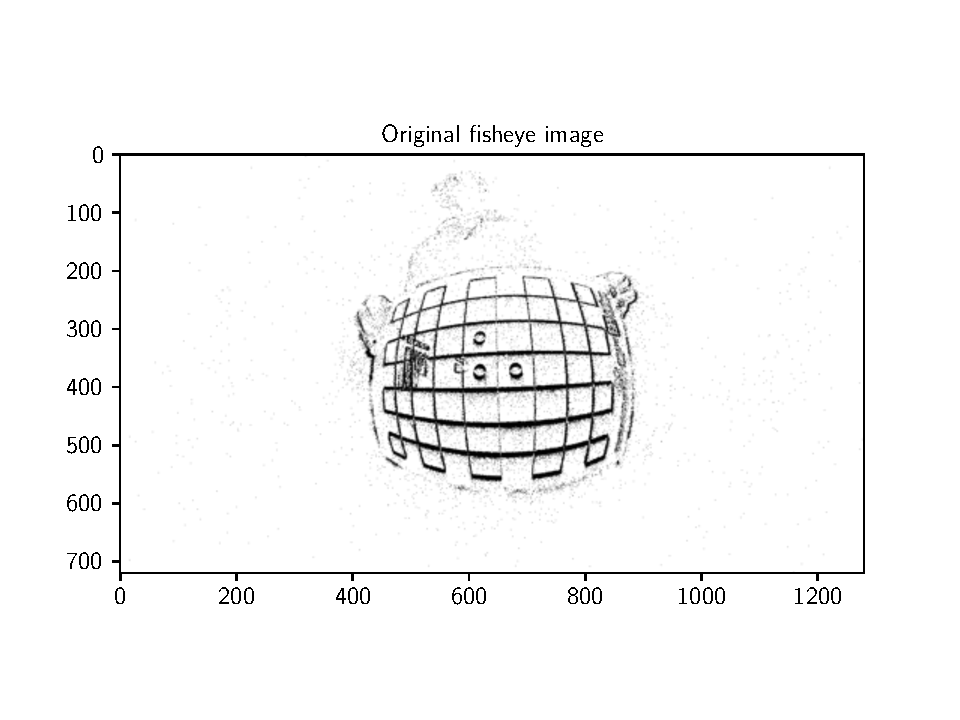
\includegraphics[width=0.5\textwidth]{./fig/pgfplot/build/ent_before.pdf}
	  \label{fig:calib_ent_proj_1}
	}
	\subfloat[Calibrated image.] {
	  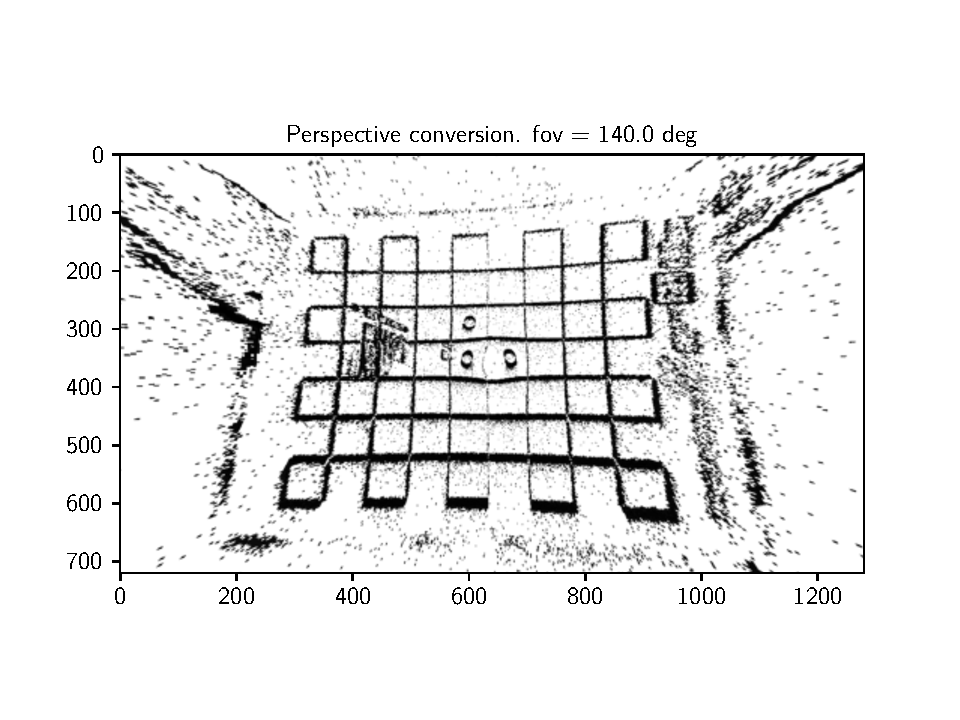
\includegraphics[width=0.5\textwidth]{./fig/pgfplot/build/ent_after.pdf}
	  \label{fig:calib_ent_proj_2}
	}
	\caption{
		Two photos of the calibration chessboard from the Entaniya 280 degree lens, one uncalibrated on \reffig{fig:calib_ent_proj_1} and the one calibrated at \reffig{fig:calib_ent_proj_1}.
  }
	\label{fig:calib_ent_proj}
\end{figure}

%\todo{change wording regarding lens FOV - inconsistent between 187 and 280 degrees (one is not the whole FOV but is mentioned as}

\section{Stationary experiments results}
For the stationary experiment a simple
\ac{PnP} (\ac{P3P}) estimation was performed with a calibrated camera, the ground truth data being the measured distance from the camera to the
stationary \ac{UAV} placed on the ground.
The results can be seen on \reffig{fig:pnpres}, with several recordings
present for each distance. The mean distance estimation error was $0.34$ meters with a standard deviation of $0.16$ meters.
\begin{figure}[H]
	\centering
	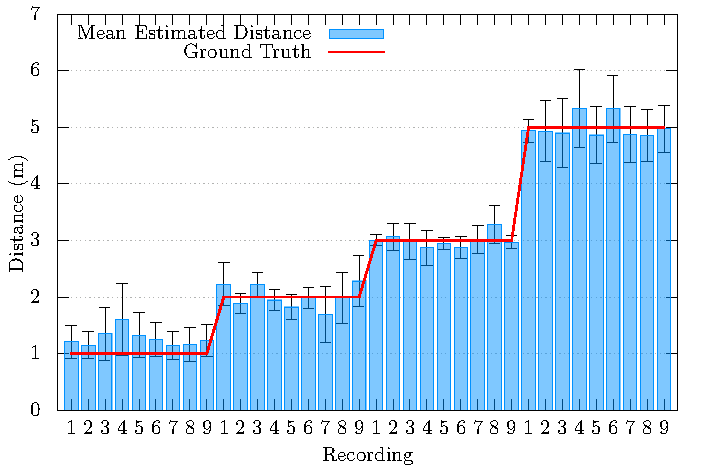
\includegraphics[width=0.75\textwidth]{./fig/tikz/pnp_results.pdf}
	\caption{PnP estimation results}
	\label{fig:pnpres}
\end{figure}

\section{Real-world experiment results}

The data was analyzed after the recording, by generating image frames from the raw event recordings, which
were synchronized to the recorded data in the ROS bags.
The generated images, as seen on \reffig{fig:labeled}, have then been manually labeled and with the use of a blob detector
the \ac{LED} sources
were selected. For each of the selected blobs, a center was then selected by calculating the closest pixel to the
blob's centroid.

\begin{figure}[H]
	\centering
	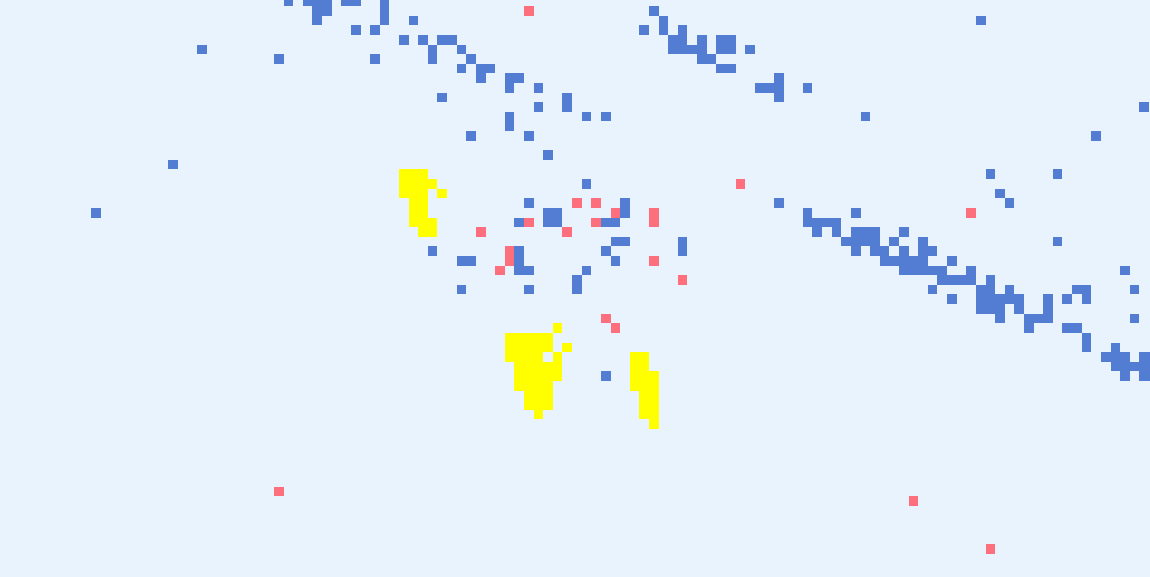
\includegraphics[width=0.7\textwidth]{./fig/photos/labeled_2.png}
	\caption{Labeled blob centers}
	\label{fig:labeled}
\end{figure}

For each group of labeled points, a distance estimation was performed with the \texttt{DistanceEstimator} ROS node using the
\ac{P3P} algorithm. For each estimated pose, a distance from the camera was calculated, which was then compared to the
ground truth distance obtained from the \ac{GNSS}. The distance is calculated as a norm of the difference of the \ac{UAV} positions.
The results demonstrate that our approach achieves a mean absolute error of $2.47$ meters, with a standard deviation of $1.75$ meters,
indicating moderate precision under the experiment conditions.
The distance estimation
results can be seen on \reffig{fig:experiment_results} with the estimated pose results visible on \reffig{fig:3dp}.

\begin{figure}[H]
	\centering
	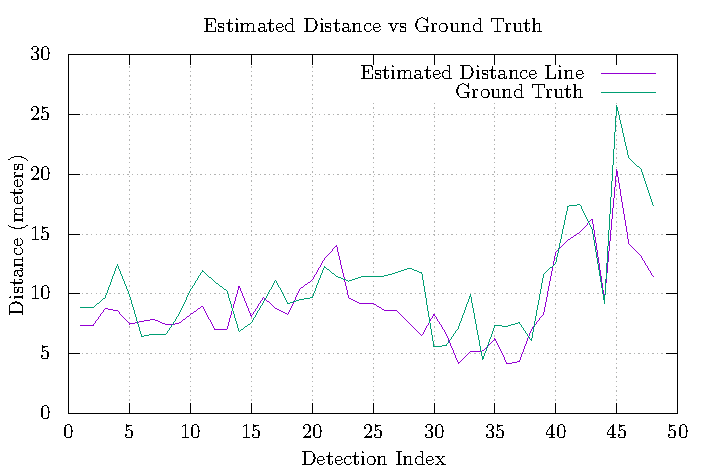
\includegraphics[width=0.7\textwidth]{./fig/tikz/experiment_analysis.pdf}
	\caption{The distance estimation data from the experiment, compared with the recorded GNSS data used as ground truth}
	\label{fig:experiment_results}
\end{figure}

\begin{figure}[H]
    \centering
    %\subfloat[$10$ Hz blinking frequency] {
    %    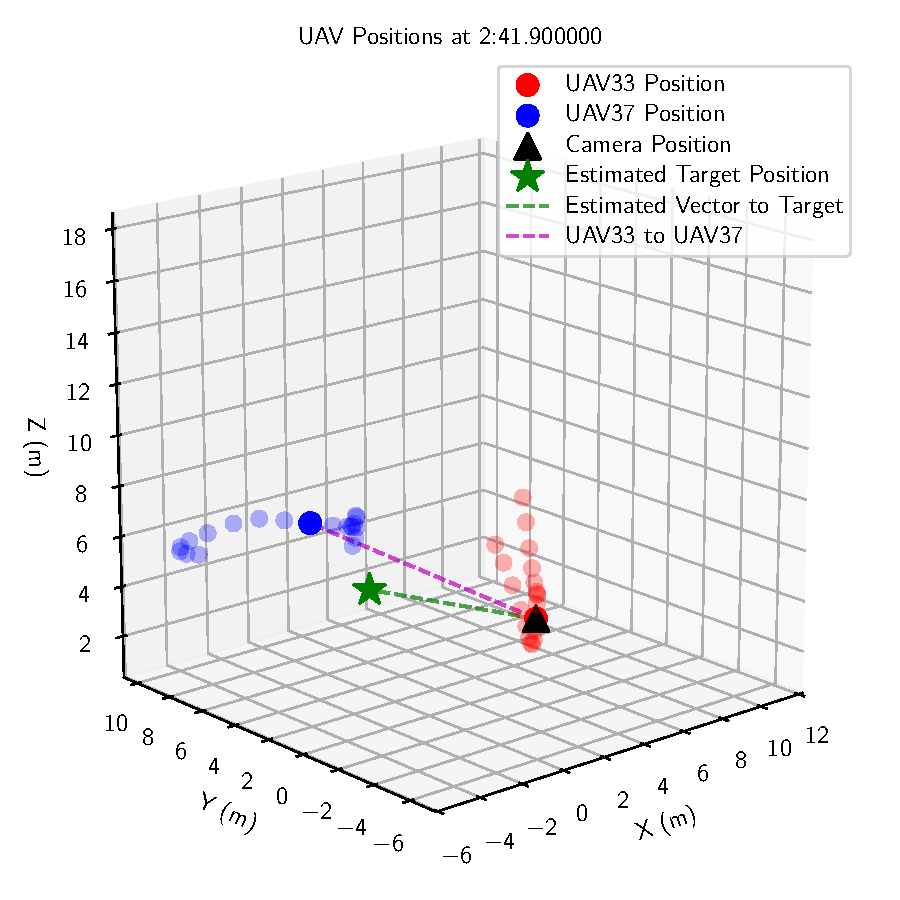
\includegraphics[width=0.33\textwidth]{./fig/pgfplot/build/3dplot1.pdf}
    %    \label{fig:freqsi_1}
    %}
    \subfloat[Fist pose estimation] {
        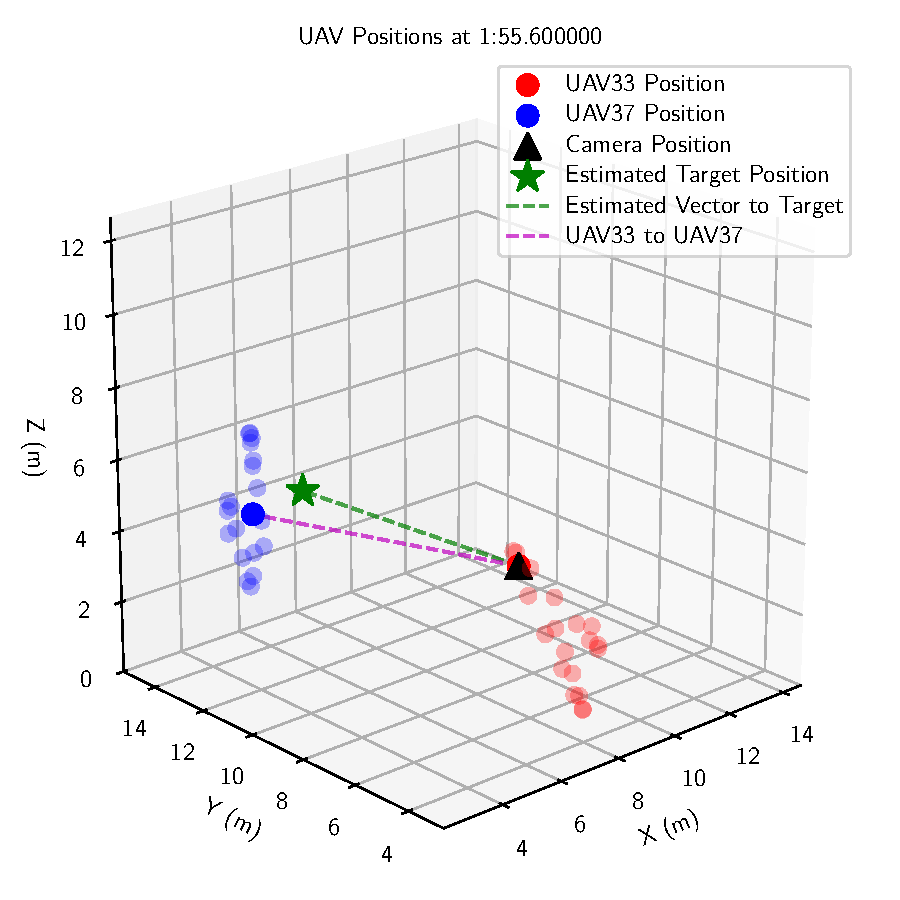
\includegraphics[width=0.5\textwidth]{./fig/pgfplot/build/3dplot2.pdf}
        \label{fig:3dp_1}
    }
    \subfloat[Second pose estimation] {
        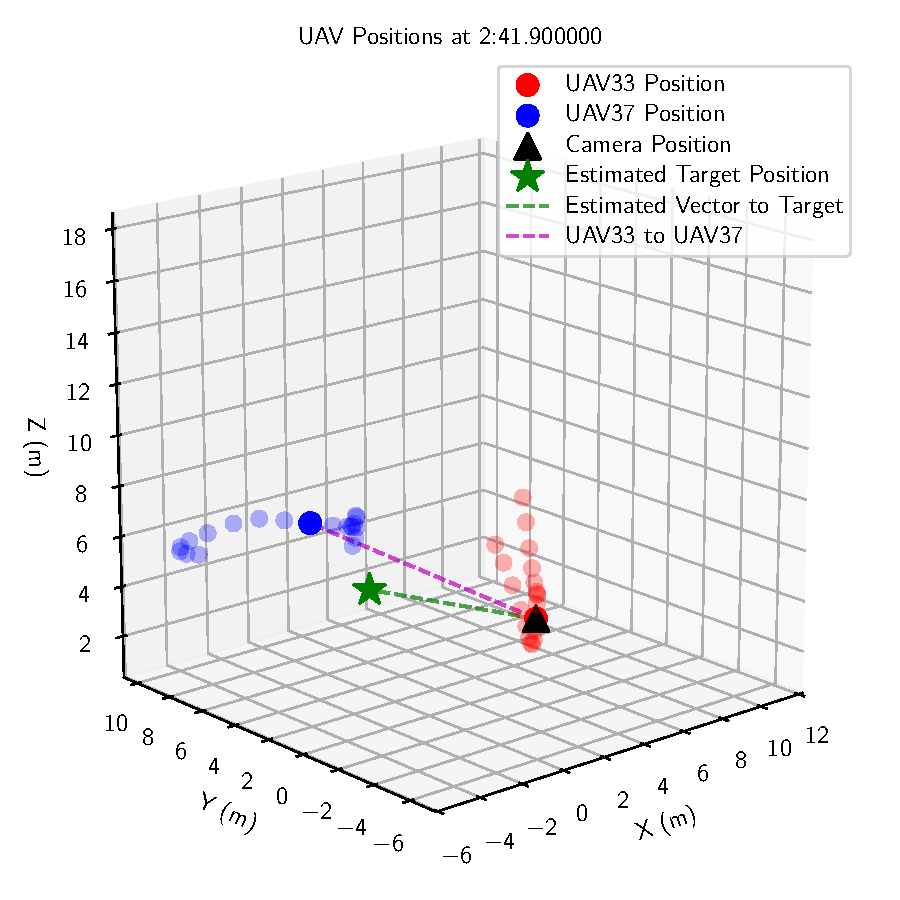
\includegraphics[width=0.5\textwidth]{./fig/pgfplot/build/3dplot1.pdf}
        \label{fig:3dp_2}
    }
    \caption{
        The estimated poses of UAV37 at two different timestamps at \reffig{fig:3dp_1} and \reffig{fig:3dp_2}, with the \ac{UAV} trajectories for UAV33 highlighted in red and for UAV37 highlighted in blue.
    }
\label{fig:3dp}
\end{figure}

\section{Real-life deployment - estimation challenges}

The analysis presents several challenges, one of them being the identification of the moving \ac{UAV} in the recorded
data. The ideal solution is to identify which pixels are being generated with their specific frequeny, which the \ac{LED}
markers are set to blink on the. Sadly, during the measurement of our experiment, the \ac{UAV} produced a lot
of vibration in the data, which interfered with our measurements, and thus the detection of blobs has become a large obsacle.
When images are generated from the recording, the problem persists; How to identify the correct blobs automatically, when
the \ac{UAV} can be at an arbitrary distance and orientation?
Manual labeling is not the definitive answer to our problem either because even the blob center selection itself can greatly
influence the estimation precision. In \reffig{fig:blob_comb}, a single pixel is selected from each blob and the distance estimation is run
for each combination of pixels. As can observed, even a difference in the range of 3 pixels can change the estimated distance by
$1.5$ meters. The center of a blob may be calculated as a geometrical center of the blob's pixels, but this approach fails
when the blob contains pixels which do not belong to them. %Secondly, the calculation of the exact center would most likely yield results with sub-pixel level precision, requiring the placement of the center between the pixels

A fundamental limitation of any vision‐based positioning system is the finite spatial resolution of the camera sensor. As the distance to the \ac{LED}s increases, beyond roughly $20$ meters in our setup, their angular size on the image plane decreases to just a few pixels. Once a marker spans only a few sensor pixels, adjacent light sources can begin to merge: individual \ac{LED} spots can no longer be differentiated and their point-spread functions overlap. This blending of pixel responses prevents the reliable separation of each \ac{LED} signal and ultimately makes accurate detection and decoding impossible.

\begin{figure}[H]
	\centering
	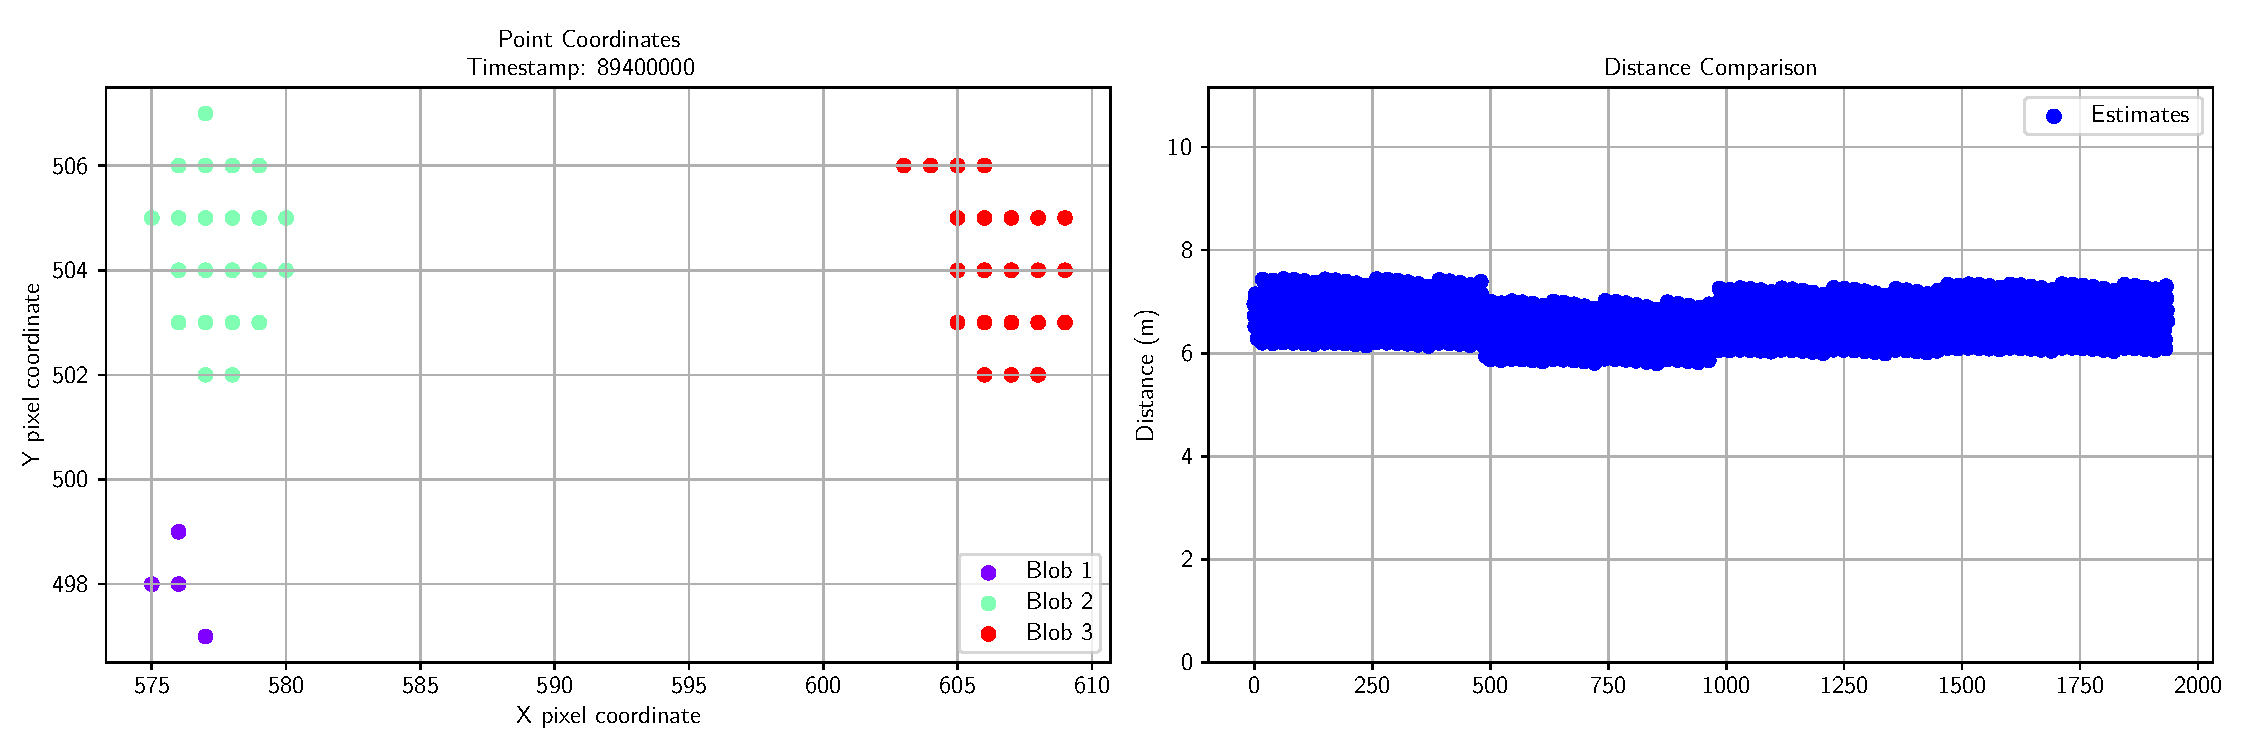
\includegraphics[width=0.99\textwidth]{./fig/pgfplot/build/estimation_selection_1.pdf}
	\caption{Blob centers with the resulting distance estimations for any combination of center selection}
	\label{fig:blob_comb}
\end{figure}
